%! TEX root = LaTeX_tips.tex

%% LaTeX tips and stuff.
%% Made for you not to spend long hours on Google and StackOverflow to look weird stuff up.
%%
%% Copyright 2020 Riccardo Milani
%%
%% Licensed under the "THE BEER-WARE LICENSE" (Revision 42):
%% Riccardo Milani wrote this file. As long as you retain this notice you
%% can do whatever you want with this stuff. If we meet some day, and you think
%% this stuff is worth it, you can buy me a beer or coffee in return


% Authors: Riccardo Milani, X12

% Acknowledgments: Cl\'ement Colas, Ga\"etan Mangeon, Germain Davy

\documentclass[a4paper,12pt,%
              final%
              %draft%
              ]{article}

\usepackage[english]{babel}
\usepackage[utf8]{inputenc}
\usepackage[T1]{fontenc}
%\usepackage{lmodern}

\usepackage[top=3cm, bottom=3cm, left=2cm, right=2cm]{geometry}

\usepackage{xcolor}
\definecolor{BlueX}{RGB}{0,62,92}
\def\maincolor{BlueX}
\definecolor{mLightBrown}{HTML}{EB811B}

\usepackage{verbatim}
\usepackage{fancyvrb}

\usepackage{amsmath,amssymb,amsfonts,mathtools,amsthm}
\usepackage{empheq}

\usepackage{fontawesome}

\usepackage{lipsum}

\usepackage{paralist}

\usepackage[inline]{enumitem}
\setlist[itemize]{topsep=0pt,noitemsep}

\usepackage{xspace}

\usepackage{tikz}
\usetikzlibrary{trees}
\usepackage{forest}

\usepackage{titlesec} % Modify the style of the sections, chapters...
\titleformat{\section} %command
    %[display] %shape
    {\color{\maincolor}\Large\bfseries\itshape} %format
    {\color{\maincolor}\Large\bfseries\itshape\thesection~-} %label
    {1ex} %sep
    {} %before-code
    %{} %after-code
\titleformat{\subsection} %command
    %[display] %shape
    {\color{\maincolor}\large\bfseries} %format
    {\color{\maincolor}\large\bfseries\thesubsection~-} %label
    {.5ex} %sep
    {} %before-code
    %{} %after-code

\usepackage[%
  pdfpagelabels,
  urlbordercolor=\maincolor,
  linkbordercolor=mLightBrown,
]{hyperref}
\newcommand*{\fullref}[1]{\hyperref[{#1}]{\autoref*{#1} - \textit{\nameref*{#1}}}}

\usepackage[numbered]{bookmark}

\parindent=0pt
\setlength{\parskip}{2ex}

\title{\color{\maincolor}\Huge\bfseries\scshape Random (and possibly useful) \LaTeX{} tips}
\author{\vspace{-7ex}}
\date{\vspace{-7ex}}
\addto\captionsenglish{% Needed if babel is used. It is needed for every language that will be used.
  \renewcommand{\abstractname}{\vspace*{-\baselineskip}}%
}
%
\begin{document}

\maketitle
%\begin{center}
%{\color{\maincolor}\Huge\bfseries\scshape%
  %Random (and possibly useful) \LaTeX~tips}
%\end{center}
\vspace*{-2,5cm}

\pdfbookmark[1]{Abstract}{abstract}
\begin{abstract}
\parindent=0pt
\setlength{\parskip}{2pt}
\noindent We collect here some \LaTeX{} tricks that we used (do not ask why) and that we found useful. We hope that this list could save some Googlin', roaming around StackExchange and, most importantly, time to other people who may happen to need the same things.

Indeed, this is not a tutorial, this is not an introduction to \LaTeX{}, we assume that the reader has already some (basic) notions. In particular, [s]he should be able to write and compile properly a \texttt{tex} file. You may find here and there some basic stuff (for instance the chain of commands to obtained a fully compiled file), but it won't suffice if you start with zero knowledge of \LaTeX{}. The usual tools (namely Google) is your friend.

There is no particular structure or whatsoever. We identified some major themes and then simply put an itemize in there. A brief ToC is given here below.

We try to give the snippet of the solution, hopefully commented, and an example: please copy them, and play around with them in order to make them suit your desires! If a loading of a package is required, you'll often see \verb|%...| or alike, usually meaning that what comes before it, goes in the preamble, what comes next into the document. Sometimes, when we were too lazy and we found it pretty clear, a link to an on-line solution is given. In our snippets, you'll find words in \texttt{< >}, that means that it is something that you have to / can choose. When discussing a package, we often provide the link to the PDF of the user manual: this might change and not be accessible anymore, if that happens, just google "in:ctan.org <name\_of\_the\_package>" and open the related \href{https://ctan.org/}{CTAN} (Comprehensive \TeX{} Archive Network) address, and please, modify the link in this document, or, at least, report the issue.

If one would like more details about a subject, or if [s]he couldn't find / solve his/her problem with this document, there are a couple of websites that could be useful. \href{https://ctan.org/}{CTAN}, has already been mentioned, and (all hail!) \href{https://tex.stackexchange.com/}{TexExchange} as well. Other references are: \href{https://www.tug.org/}{\TeX{} Users Group}, \href{https://www.overleaf.com/learn/}{Overleaf}, \href{https://en.wikibooks.org/wiki/LaTeX}{WikiBooks}, \href{https://latex.org/forum/index.php}{\LaTeX.org} and \href{https://www.texfaq.org/}{\TeX{} FAQ}.

A couple of words about \LaTeX{} editors. If for you writing in \LaTeX{} is a necessary pain (what's all this code anyway?!), there are plenty of dedicated editors out there that make things easy for you, among others \LaTeX Studio and \TeX Maker (see \autoref{sec:texmaker}). I think that the rich-format text option of the aforementioned \href{https://www.overleaf.com/learn/}{Overleaf} (or Share\LaTeX{} since they have merged) can definitely be a killer-feature. Overleaf might also be a good choice for a collaborative project, in this case, see the related item in \autoref{sec:Miscellaneous}. If you are more code-prone, numerous plugin have been developed for classical text editors such as \verb|[neo]vi[m]| or \verb|emacs| (I, myself, cannot but suggest \verb|vim+vimtex+Ultisnips|). One may found a list of available editors \href{https://tex.stackexchange.com/questions/339/latex-editors-ides}{here}.

Finally, if you liked and you have some cool tricks that you want to share in order to make other people's lives easier, do not hesitate to contribute: along with this file, you should have received its \href{run:./LaTeX_tips.tex}{source code} (of course we wrote it in \LaTeX, what do you expect?!); if not, ask for it (there are some tricks inside it, too!). And there's more: a Github repo. Here it is: \href{https://github.com/RiMillo/LaTeX_tips}{\faGithub\texttt{/RiMillo/LaTeX\_tips}}.

Happy \LaTeX ing! And remember: {\itshape Sharing is caring!}
\end{abstract}
%\clearpage

\tableofcontents
%\clearpage
%%%%%%%%%%%%%%%%%%%%%%%%%%%%%%%%%%%%%%%%%%%%%%%%%%%%%%%%%%%%%%%%%%%%%%%%%%%%%%%%
%%%                   SECTION: SECTIONING
%%%%%%%%%%%%%%%%%%%%%%%%%%%%%%%%%%%%%%%%%%%%%%%%%%%%%%%%%%%%%%%%%%%%%%%%%%%%%%%%
\section{Structure, Sectioning \& General Layout}
\label{sec:Sectioning}
\begin{itemize}
  \item Manage a big, multi-file project: \verb|\input| vs. \verb|\include|, \verb|\includeonly|, packages \href{https://ctan.mc1.root.project-creative.net/macros/latex/contrib/import/import.pdf}{\texttt{import}} and \href{http://mirror.ibcp.fr/pub/CTAN/macros/latex/contrib/subfiles/subfiles.pdf}{\texttt{subfiles}}; have a look \href{https://en.wikibooks.org/wiki/LaTeX/Modular_Documents}{here}.
    \begin{itemize}
      \item Nested \verb|\input| are forbidden.
      \item You may know about \verb|\graphicspath| which allows one to add directories to the path where the pictures are searched for (cf.~\fullref{sec:Graphics}). Well, with a workaround one can achieve the same thing for the input files. Details \href{https://tex.stackexchange.com/a/79060/206129}{here} but an example is given below:
\begin{verbatim}
\makeatletter
\providecommand*{\input@path}{}
\g@addto@macro\input@path{{path1/}{path2/}}% append
\makeatother
\end{verbatim}
    \end{itemize}
  \item General introduction to a structure of a document: \href{https://en.wikibooks.org/wiki/LaTeX/Document_Structure}{here}
    \begin{itemize}
      \item The \texttt{book} class has a special \href{https://en.wikibooks.org/wiki/LaTeX/Document_Structure#Book_structure}{structure}: \verb|\frontmatter|, \verb|\mainmatter|, \verb|\appendix|, \verb|\backmatter|.
    \end{itemize}
  \item You may now know that one defines a chapter with \verb|\chapter{Chpt title}|, a section with \verb|\section{Sec title}|, and similarly for \texttt{part}, \texttt{subsection}, \texttt{subsubsection}, \texttt{paragraph}, \texttt{subparagraph}. There is also the possibility to choose a "short title" and a "mark". The example here below is for \texttt{section} but can be applied to the other commands as well
\begin{verbatim}
\section[Short title]{A very long long tile: do you really want it?}
\sectionmark{Section in header}
\end{verbatim}
    \begin{itemize}
      \item Ok, you know about the braces and the long title.
      \item A short title is what will appear in the ToC (Table of Contents) (and possibly in the footer/header of a \texttt{beamer} document \autoref{sec:Beamer}).
      \item A mark is what will appear in the header/footer. Of course, there should be one and it needs the \texttt{fancyhdr} package (see here below). In the \texttt{fancyhdr} manual, the authors say it is better to repeat the \verb|\sectionmark{}| inside the long title too (let me stress: repeat, copy\ldots) in order to avoid some possible problems of undefined marks, however this seem to be possible only if a short title is provided as well.
    \end{itemize}
  \item Modify first indentation: \verb|\parindent=<len>|
  \item Customize titling style: package \href{http://mirrors.ircam.fr/pub/CTAN/macros/latex/contrib/titlesec/titlesec.pdf}{\texttt{titlesec}}; an example
\begin{Verbatim}[samepage=true]
\titleformat{\section} % Command: chapter, subsection...
    %[display] % Shape - Optional
    {\color{\maincolor}\Large\bfseries\itshape} % Format
    {\color{\maincolor}\Large\bfseries\itshape\thesection~-} % Label
    {1ex} % Separation
    {}    % Before-code
    %{}   % After-code - Optional
\end{Verbatim}
  \item Indent first line after section. Depending on (the typographic rules of) the chosen language, the first line after a non-centered titled \emph{section} may not be indented. If you would like to indent it anyway, just load \verb|\usepackage{indentfirst}|.
  \item Indent a \emph{whole} paragraph: have a look \href{https://tex.stackexchange.com/questions/35933/indenting-a-whole-paragraph}{here}.
  \item Numbering and ToC depth (how many levels are printed):
    \begin{itemize}
      \item \verb|\seccounter{secnumdepth}<n>|: define up to which level of sectioning titles are numbered.
      \item \verb|\setcounter{tocdepth}{<n>}| (mind that you can change the numbered level with \verb|\setcounter{secnumdepth}{<n>}| so that they are included in the ToC, but it is not exactly the same thing, as it is explained \href{https://tex.stackexchange.com/questions/17877/how-to-show-subsubsections-and-paragraphs-in-toc/17879#17879}{here}).
      \item Selectively change the depth: have a look \href{https://en.wikibooks.org/wiki/LaTeX/Document_Structure#Table_of_contents}{here} or \href{https://tex.stackexchange.com/questions/59091/setcountertocdepth}{here}.
    \end{itemize}
  \item If the ToC does not show up in the bookmarks, you can add it manually. Just remember to add a \verb|\clearpage| or \verb|\cleardoublepage| just before it, so that the page in the bookmark is not messed up (we use \texttt{chapter} as level of the related ToC entry, but you can use \texttt{section} or whatever)
\begin{verbatim}
\cleardoublepage
\pdfbookmark[chapter]{\contentsname}{toc}
\tableofcontents
\end{verbatim}
  \item Lengths and skips: \href{https://tex.stackexchange.com/questions/41476/lengths-and-when-to-use-them}{here}.
  \item Horizontal / landscape pages
    \begin{itemize}
      \item For the whole document: use option \texttt{landscape} \verb|\usepackage[landscape]{geometry}| or \verb|\documentclass[landscape]{<class>}|.
      \item For a certain part only: have a look \href{https://tex.stackexchange.com/questions/337/how-to-change-certain-pages-into-landscape-portrait-mode}{here}. The environment is only one \verb|\begin{landscape}|, but it could come from two packages. If you are producing a pdf, use package \texttt{pdflscape} (it gives more metadata to the document that improve its readability), otherwise \texttt{lscape}.
        \begin{itemize}
          \item For horizontal numbering as well, see \href{https://tex.stackexchange.com/questions/9071/how-to-translate-and-rotate-the-heading-of-landscaped-pages}{this}.
        \end{itemize}
    \end{itemize}
  \item Footnotes: \verb|\footnote{This goes in the footer}|. You may want to customize the appearance, have a look \href{https://www.overleaf.com/learn/latex/footnotes#Changing_the_numbering_style}{here}. For advanced customization, refer to package \href{http://ctan.mines-albi.fr/macros/latex/contrib/footmisc/footmisc.pdf}{\texttt{footmisc}}.
    \begin{itemize}
      \item ATTENTION: \texttt{beamer} (\autoref{sec:Beamer}) defines its own \texttt{footnote}, hence it could be used with \texttt{footmisc}. If you want to change the behaviour you should redefine the template:
\begin{verbatim}
\setbeamertemplate{footnote}{...}
\end{verbatim}
    \end{itemize}
  \item Customize headers and footers: package \href{http://mirrors.standaloneinstaller.com/ctan/macros/latex/contrib/fancyhdr/fancyhdr.pdf}{\texttt{fancyhdr}}.
\end{itemize}

%%%%%%%%%%%%%%%%%%%%%%%%%%%%%%%%%%%%%%%%%%%%%%%%%%%%%%%%%%%%%%%%%%%%%%%%%%%%%%%%
%%%                   SECTION: FONT & APPEARANCE
%%%%%%%%%%%%%%%%%%%%%%%%%%%%%%%%%%%%%%%%%%%%%%%%%%%%%%%%%%%%%%%%%%%%%%%%%%%%%%%%
\section{Font, Appearance \& Spacing}
\label{sec:font}
\begin{itemize}
  \item \href{https://en.wikibooks.org/wiki/LaTeX/Fonts}{A general intro}.
  \item Font-related
    \begin{itemize}
      \item Be advised: changing the font appearance with \LaTeX{} may be hard. There are some predefined ones, you may find them \href{https://www.overleaf.com/learn/latex/font_typefaces}{here}, but there are only a dozen. If you want a new style you should install it, look it up on the web, you can start \href{https://tug.org/fonts/fontinstall.html}{here}. It is easier if one uses Xe\LaTeX{}.
      \item Be advised that \verb|\emph{.}| does not not necessarily means italic. You might modify it as reported \href{https://tex.stackexchange.com/questions/315058/change-the-behaviour-of-emph-per-environment}{here} or \href{https://tex.stackexchange.com/questions/315058/change-the-behaviour-of-emph-per-environment}{here}.
      \item Change default font style: \verb|\renewcommand{\familydefault}{<family>}| where \texttt{family} may be chosen in: \verb|\rmdefault| {roman family font}, \verb|\sfdefault| (sans serif family font), or \verb|\ttdefault| (teletype font family)
      \item Font sizes: see \autoref{tab:sizes}. Note: \verb|\HUGE| is available with the \texttt{memoir} class only, \verb|\Tiny| and \verb|\TYNY| only with \texttt{beamer}.
      \item Font styles: see \autoref{tab:styles}.
    \end{itemize}
  \item \LaTeX{} lengths: have a look \href{https://www.overleaf.com/learn/latex/Lengths_in_LaTeX}{here} or even \href{https://en.wikibooks.org/wiki/LaTeX/Lengths}{there}.
  \item Spacing:
  \begin{itemize}
    \item \verb|\vspace{<length>}| (resp.~\verb|\hspace{<length>}|) tells \LaTeX{} to leave a vertical (resp.~horizontal) space. Its starred version \verb|\vspace*{<len>}| forces it when you are close to the top/bottom of the page.
    \item For leaving one-time space between two lines, use \verb|\smallskip|, \verb|\medskip| or \verb|\bigskip| (which are equivalent to e.g.~\verb|\vspace{\smallskipamount}|).
    \item \verb!\small|med|bigbreak!: as above but suggests to \LaTeX{} that it would be a good place for a pagebreak if necessary.
    \item When forcing a newline, a custom vertical space may be added: \verb|The end\\[3cm]|.
    \item Fill the line/page: \verb!\hfill!, \verb!\vfill!. Might be useful: for lines \verb|\dotfill|, \verb|\hrulefill|.
    \item Change the space after paragraph: \verb|\setlegth{\parskip}{<len>}|
    \item Spacing after a command
      \begin{itemize}
        \item Use a user-defined command and empty brackets as suggested \href{https://tex.stackexchange.com/questions/31091/space-after-latex-commands}{here}. Examples:
  \newcommand{\cmd}{command}
\begin{verbatim}
\newcommand{\cmd}{command}
A space after my \cmd{} here. There shouldn't be one after my \cmd{}.
\end{verbatim}
        gives:\\
        A space after my \cmd{} here. There shouldn't be one after my \cmd{}.
        \item Use package \texttt{xspace} as explained \href{https://tex.stackexchange.com/questions/362046/insert-a-space-after-a-command-vs-vs-space}{here}.
  \newcommand{\cmdd}{command\xspace}
\begin{verbatim}
\usepackage{xspace}
\newcommand{\cmd}{command\xspace}
A space after my \cmd here. There shouldn't be one after my \cmd.
\end{verbatim}
        A space after my \cmdd{} here. There shouldn't be one after my \cmdd{}.
      \end{itemize}
  \end{itemize}
  \item Special and Accented characters: \href{https://en.wikibooks.org/wiki/LaTeX/Special_Characters#Escaped_codes}{here} (the link is useful for other symbols as well).
  \item Special styles, e.g.~underlined, highlighted, spaced-out\ldots{}
    \begin{itemize}
      \item The package \href{https://mirrors.chevalier.io/CTAN/macros/latex/contrib/ulem/ulem.pdf}{\texttt{ulem}} provides several underlined styles (double, wavy, strike-out\ldots).
        \begin{itemize}
          \item It redefines the \verb|\emph{[...]}| command to underlined (instead of italic). Add option \texttt{normalem} to avoid that: \verb|\usepackage[normalem]{ulem}|.
        \end{itemize}
      \item The package \href{http://ctan.tetaneutral.net/macros/latex/contrib/soul/soul.pdf}{\texttt{soul}} gives interesting hyphenatable (can be cut to go to next line) styles: spaced-out, highlighted, underlined\ldots{}
    \end{itemize}
  \item (Semi-)Transparent text: obtaining a faded text is easy in \texttt{TikZ} (\autoref{sec:tikzpgf}): use option \verb|opacity=<r>| where \texttt{r} is a number between 0 (completely transparent) and 1 (solid). Some others options are available for standard text. The dedicated package \href{http://ctan.mines-albi.fr/macros/latex/contrib/transparent/transparent.pdf}{\texttt{transparent}} with \verb|\transparentcolor{<r>}{<text>}|, or the first two answers of this \href{https://stackoverflow.com/questions/3594329/semi-transparent-text-in-beamer-pdflatex}{post}.
  \item Poetry: reference packages \href{https://ctan.gutenberg.eu.org/macros/latex/contrib/verse/verse.pdf}{\texttt{verse}} (pretty basic but it does the job; it seems to be frozen) and \href{https://mirrors.chevalier.io/CTAN/macros/latex/contrib/poemscol/poemscol.pdf}{\texttt{poemscol}} (a complete and huge package).
\end{itemize}
\begin{table}
  \centering
  \caption{Font sizes}
  \label{tab:sizes}
  \begin{tabular}{lc}
    \verb|\HUGE|         & [\texttt{memoir} only]\\
    \verb|\Huge|         & {\Huge         The quick brown fox\par}\\
    \verb|\huge|         & {\huge         The quick brown fox\par}\\
    \verb|\LARGE|        & {\LARGE        The quick brown fox\par}\\
    \verb|\Large|        & {\Large        The quick brown fox\par}\\
    \verb|\large|        & {\large        The quick brown fox\par}\\
    \verb|\normalsize|   & {\normalsize   The quick brown fox\par}\\
    \verb|\small|        & {\small        The quick brown fox\par}\\
    \verb|\footnotesize| & {\footnotesize The quick brown fox\par}\\
    \verb|\scriptsize|   & {\scriptsize   The quick brown fox\par}\\
    \verb|\tiny|         & {\tiny         The quick brown fox\par}\\
    \verb|\Tiny|         & [\texttt{beamer} only]\\
    \verb|\TINY|         & [\texttt{beamer} only]\\
  \end{tabular}
\end{table}
\begin{table}
  \centering
  \caption{Font styles}
  \label{tab:styles}
  \begin{tabular}{lll}
    Command & Switch & Output \\
    \hline
    \verb|\textnormal{...}| & \verb|{\normalfont ...}| & \textnormal{document font family}\\
    \verb|\emph{...}| & \verb|{\em ...}| & \emph{emphasis}\\
    \verb|\textrm{...}| & \verb|{\rmfamily ...}| & \textrm{roman font family}\\
    \verb|\textsf{...}| & \verb|{\sffamily ...}| & \textsf{sans serif font family}\\
    \verb|\texttt{...}| & \verb|{\ttfamily ...}| & \texttt{teletype font family}\\
    \verb|\textup{...}| & \verb|{\upshape ...}| & \textup{upright shape}\\
    \verb|\textit{...}| & \verb|{\itshape ...}| & \textit{italic shape}\\
    \verb|\textsl{...}| & \verb|{\slshape ...}| & \textsl{slanted shape}\\
    \verb|\textsc{...}| & \verb|{\scshape ...}| & \textsc{Small Capitals}\\
    \verb|\textbf{...}| & \verb|{\bfseries ...}| & \textbf{bold}\\
    \verb|\textmd{...}| & \verb|{\mdseries ...}| & \textmd{medium weight, normal}\\
    %\verb|\textlf{...}| & \verb|{\lfseries ...}| & \textlf{light}\\
    \verb|\uppercase{...}| &  & \uppercase{All caps}\\
    \verb|\lowercase{...}| &  & \lowercase{LOWER CAPS}
  \end{tabular}
\end{table}

%%%%%%%%%%%%%%%%%%%%%%%%%%%%%%%%%%%%%%%%%%%%%%%%%%%%%%%%%%%%%%%%%%%%%%%%%%%%%%%%
%%%                   SECTION: LANGUAGES
%%%%%%%%%%%%%%%%%%%%%%%%%%%%%%%%%%%%%%%%%%%%%%%%%%%%%%%%%%%%%%%%%%%%%%%%%%%%%%%%
\section{Languages}
\label{sec:languages}
Sometimes, especially in a thesis, one may have to use different languages, possibly with different typesetting styles (e.g.~white-space before semicolon in French not in English). \href{https://en.wikibooks.org/wiki/LaTeX/Internationalization}{Here}, one can find an article about the internalization with pieces of advice and examples. When juggling more than one languages, the \texttt{babel} package comes in hand.
\begin{itemize}
  \item Load the \texttt{babel} package with the languages you want to use as options. The order is important since the last one is considered as default one:
\begin{verbatim}
\usepackage[<secondary_language>,<main_language>]{babel}
\end{verbatim}
  Thus, if one want to use French and English with the latter as default one would write \verb|\usepackage[french,english]{babel}|
  Even simpler, use the key \texttt{main}:
\begin{verbatim}
 \usepackage[french,main=english]{babel}
\end{verbatim}
  \item When a paragraph should be typeset / written in French, one should just switches the language with the help of the \texttt{otherlanguage} environment (an example \href{https://tex.stackexchange.com/questions/20987/changing-babel-package-inside-a-single-chapter}{here}):
\begin{Verbatim}[samepage=true]
[English typesetting]
\begin{otherlanguage}{french}
[French typesetting]
\end{otherlanguage}
[English typesetting]
\end{Verbatim}
  \item For some languages (e.g.~Italian) \texttt{babel} changes autonomously caption names (figure, table,\ldots) and stuff (table of contents\ldots). With \texttt{french} (and similar) this does not happen for everything, hence one may want to rename manually the captions. For instance, one can use: \verb|\addto\captionsfrench{\def\tablename{Tableau}}|.
  \item When certain languages are loaded, \texttt{babel} may be incompatible with some packages. This comes down to the fact that it modifies basic characters. Think about the semicolon ``\texttt{;}'' which in French gets modified so that a thin space is added before it. There are packages (for instance, \texttt{tikz}, see \autoref{sec:tikzpgf}) which suppose that such character have its basic and original meaning. This may cause compatibility issues. If you fear that a certain error is due to this incompatibility, you can try to switch off the particular value of the character, with \verb|\shorthandoff{;}|. You may reactivate it with \verb|\shorthandon{;}|. Other incompatibilities may involve Spanish and German, and characters like ``!'', ``>'', ``<'', ``:''.
\end{itemize}

%%%%%%%%%%%%%%%%%%%%%%%%%%%%%%%%%%%%%%%%%%%%%%%%%%%%%%%%%%%%%%%%%%%%%%%%%%%%%%%%
%%%                   SECTION: ITEMIZE & Co.
%%%%%%%%%%%%%%%%%%%%%%%%%%%%%%%%%%%%%%%%%%%%%%%%%%%%%%%%%%%%%%%%%%%%%%%%%%%%%%%%
\section{Items \& Co.}
\label{sec:Items}
\begin{itemize}
  \item In \texttt{enumerate} start from a different number: just add \verb|\setcounter{enumi}{<n>}| (as proposed \href{https://overleaf.com/learn/latex/Counters}{here}). See also below with package \texttt{enumitem} and \autoref{sec:Miscellaneous} for managing counters.
  \item The \texttt{enumitem} \href{https://ctan.crest.fr/tex-archive/macros/latex/contrib/enumitem/enumitem.pdf}{package} enables more control on the \texttt{itemize} environment and alike.
    \begin{itemize}
      \item Usage
        \begin{itemize}
          \item Locally
\begin{verbatim}
\usepackage{enumitem}
% [...]
\begin{itemize}[<options>]
  \item [...]
\end{itemize}
\end{verbatim}
          \item Globally
\begin{verbatim}
\usepackage{enumitem}
\setlist[itemize]{<options>}
\end{verbatim}
        \end{itemize}
      \item Spacing
        \begin{itemize}
          \item No indent: \texttt{leftmargin=*};
          \item No separations between items: \texttt{noitemsep};
          \item No separations whatsoever: \texttt{nosep};
          \item Modify top spacing: \texttt{topsep=<len>};
        \end{itemize}
      \item Modify the bullet: \texttt{label=<cmd>}. With a star, \texttt{label*=<cmd>}, \texttt{cmd} is repeated two times for sub-items, three for sub-sub-items, etc;
      \item Modify the numbering:
        \begin{itemize}
          \item Enumerations starting from \texttt{<n>}: \verb|\begin{enumerate}[start=<n>]|
          \item Resume the previous count: \verb|\begin{enumerate}[resume]|
        \end{itemize}
      \item Run a bit of code before/after the \texttt{itemize}: \texttt{before|after=<code>}
      \item \verb|\setlist[<type>[,<depth>]]{<options>}|: in the preamble, and will set the global parameter for all the \texttt{type}-lists of depth \texttt{depth}. If \texttt{depth} is not given, the options are set to all (sub)-items. \texttt{type} may be \texttt{itemize,description,enumerate}...
\begin{verbatim}
\setlist[itemize]{%
  leftmargin=*} % No margin for all the items of itemize
\setlist[itemize,1]{%
  label=$\bullet$} % Items are circles
\setlist[itemize,2]{%
  label=$\triangleleft$} % Sub-items are left-facing triangles
\end{verbatim}
      \item Enumerations with a prefix: \href{https://tex.stackexchange.com/questions/37740/enumerate-with-properties}{here}. Just set the label as you wish as option:
\begin{verbatim}
\begin{enumerate}[label=\textbf{H\arabic*}]
  \item Property 1
  \item Property 2
\end{enumerate}
\end{verbatim}
      \item \textbf{ATTENTION}: it may interfere with \texttt{beamer} and they may not work as expected if loaded together, see this \href{https://tex.stackexchange.com/questions/24371/does-enumitem-conflict-with-beamer-for-lists}{post} for two common problems.
      \item \textbf{ATTENTION}: it may cause some errors with the \texttt{enumerate} lists. In this case, load the option \texttt{shortlabels} and explicitly choose the type of item for the numeration
\begin{verbatim}
\usepackage[shortlabels]{enumitem}
% [...]
\begin{enumerate}[1.]
  \item One.
\end{enumerate}
\end{verbatim}
    \end{itemize}
  \item Inline lists: \href{https://mirrors.chevalier.io/CTAN/macros/latex/contrib/paralist/paralist.pdf}{\texttt{paralist}} package, and in particular its \texttt{inparaenum} environment.
    \begin{itemize}
      \item \textbf{ATTENTION}: load \texttt{paralist} \emph{before} \texttt{enumitem}.
      \item A similar result is obtained with the \texttt{inline} option of \texttt{enumitem} and using starred versions of the usual item-related environments. Consider the following example in which we set the type of label, the separator, internal and final. Here is how it appears:
        \begin{enumerate*}[label={(Ex\arabic*)},itemjoin={{, }},itemjoin*={{, and }}]
          \item Example 1
          \item Example 2
          \item Example 3
        \end{enumerate*}.
\begin{verbatim}
\begin{enumerate*}[%
  label={(Ex\arabic*)},itemjoin={{, }},itemjoin*={{, and }}]
    \item Example 1
    \item Example 2
    \item Example 3
\end{enumerate*}.
\end{verbatim}
      \item \texttt{paralist} does not work properly with \texttt{beamer}.
    \end{itemize}
  \item Referencing and \texttt{itemize}
    \begin{itemize}
      \item There is no point (actually, no way neither) in referencing an item in an \texttt{itemize}: they all look the same, you can not tell them apart;
      \item \texttt{enumerate} items can be referenced by default with the \texttt{enumitem} package, an example \href{https://tex.stackexchange.com/questions/58713/ref-should-use-enumerate-label-name}{here};
      \item For \texttt{description} items:
\begin{Verbatim}[samepage=true]
\usepackage{enumitem, hyperref}
\makeatletter
\def\namedlabel#1#2{\begingroup
    #2%
    \def\@currentlabel{#2}%
    \phantomsection\label{#1}\endgroup
}
 %...
\begin{description}[style=multiline, labelwidth=1.5cm]
    \item[\namedlabel{itm:rule1}{Rule1}] What should I do?
    \item[\namedlabel{itm:rule2}{Rule2}] Reference to \ref{itm:Rule1}
\end{description}
\end{Verbatim}
    \end{itemize}
\end{itemize}

%%%%%%%%%%%%%%%%%%%%%%%%%%%%%%%%%%%%%%%%%%%%%%%%%%%%%%%%%%%%%%%%%%%%%%%%%%%%%%%%
%%%                   SECTION: TABLES
%%%%%%%%%%%%%%%%%%%%%%%%%%%%%%%%%%%%%%%%%%%%%%%%%%%%%%%%%%%%%%%%%%%%%%%%%%%%%%%%
\section{Tables}
\label{sec:Tables}
\begin{itemize}
  \item General info \href{https://en.wikibooks.org/wiki/LaTeX/Tables}{here}
  \item Position of a table: usually a \texttt{tabular} object is loaded in a \texttt{table} environment, making it a float, that is an element whose position may not be exactly where it is typed, but it is chosen by an internal \TeX{} algorithm. This can be frustrating, I know, just be patient. Some hints about positioning are in \fullref{sec:Floats}.
    \begin{itemize}
      \item One of the main uses of the \texttt{table} environment is explicitly to make a \texttt{tabular} a float, so that, for instance, a caption (with the \verb|\caption| command) may be added
    \end{itemize}
  \item \verb|@{<ex>}|: put \texttt{<ex>} at the beginning of the following column on every row
\begin{verbatim}
\begin{tabular}{c@{:}c}
   Test  &  Test \\
  ReTest & ReTest
\end{tabular}
\end{verbatim}
\begin{itemize}
  \item \verb|@{}|: set the space between two columns to zero
\end{itemize}
    \item Fix a table width, you have to use at least once the column type \texttt{X}:
\begin{verbatim}
\usepackage{tabularx}
%...
\begin{tabularx}{<tablewidth>}{XX}
   Test  &  Test \\
  ReTest & ReTest
\end{tabularx}
\end{verbatim}
    \begin{itemize}
      \item Centered \texttt{X}-like column type: \href{https://tex.stackexchange.com/questions/89166/centering-in-tabularx-and-x-columns}{here}
\begin{verbatim}
\newcolumntype{Y}{>{\centering\arraybackslash}X}
\end{verbatim}
    \end{itemize}
  \item Merge cells: multirow \& multicolumn. Attention: multirow needs the \texttt{multirow} package
\begin{verbatim}
\multicolumn{<#cols to merge>}{<type>}{<content>}
\multirow{<#rows to merge>}{<width(or *)>}{<content>}
\end{verbatim}
    e.g.:~\verb!\multicolumn{2}{c|}{Two columns in one}!
  \item Horizontal tables / landscape: use the environment \texttt{sidewaystable} (instead of \texttt{table}) from the package \texttt{rotating}. Other solution found \href{http://distrib-coffee.ipsl.jussieu.fr/pub/mirrors/ctan/macros/latex/required/tools/longtable.pdf}{here};
  \item Wider choice of row / column separators: see package
    \href{http://distrib-coffee.ipsl.jussieu.fr/pub/mirrors/ctan/macros/latex/required/tools/longtable.pdf}{\texttt{hhline}}, or \href{https://ctan.crest.fr/tex-archive/macros/latex/contrib/arydshln/arydshln-man.pdf}{\texttt{arydshln}};
  \item Tables spanning more than one pages: use package \href{http://distrib-coffee.ipsl.jussieu.fr/pub/mirrors/ctan/macros/latex/required/tools/longtable.pdf}{\texttt{longtable}};
  \item Table and colors:
    \begin{itemize}
      \item the reference is \href{http://mirrors.ircam.fr/pub/CTAN/macros/latex/contrib/colortbl/colortbl.pdf}{\texttt{colortbl}} (which may be loaded by passing options \texttt{tables} to package \href{http://mirrors.standaloneinstaller.com/ctan/macros/latex/contrib/xcolor/xcolor.pdf}{\texttt{xcolor}}).
      \item Some tips \href{https://texblog.org/2011/04/19/highlight-table-rowscolumns-with-color}{here}.
      \item Alternate color row: see \href{https://texblog.org/2011/09/02/coloring-every-alternate-table-row/}{here}.
    \end{itemize}
  \item For typesetting numerical data (but not necessarily), you may want to have a look at \texttt{pgfplotstable}, \autoref{sec:tikzpgf}.
  \item Colored and rounded tables (use of \texttt{TikZ}, \autoref{sec:tikzpgf}): some tips \href{https://tex.stackexchange.com/a/184075}{here} and example in \href{run:./ex_plot.tex}{\texttt{ex\_plot.tex}}.
\end{itemize}

%%%%%%%%%%%%%%%%%%%%%%%%%%%%%%%%%%%%%%%%%%%%%%%%%%%%%%%%%%%%%%%%%%%%%%%%%%%%%%%%
%%%                   SECTION: GRAPHICS
%%%%%%%%%%%%%%%%%%%%%%%%%%%%%%%%%%%%%%%%%%%%%%%%%%%%%%%%%%%%%%%%%%%%%%%%%%%%%%%%
\section{Graphics \& Animations}
\label{sec:Graphics}
\begin{itemize}
  \item Into to figures and tables (and floats) management \href{https://en.wikibooks.org/wiki/LaTeX/Floats,_Figures_and_Captions}{here} or \href{https://www.overleaf.com/learn/latex/Inserting_Images}{here}.
  \item Set the path for the pictures (the directory where the pictures are searched for): from the \href{http://distrib-coffee.ipsl.jussieu.fr/pub/mirrors/ctan/macros/latex/required/graphics/grfguide.pdf}{\texttt{graphicx}} package \verb|\graphicspath{{pic_dir/}{dir2/}}|.
  \item Position of an image: usually an image is loaded in a \texttt{figure} environment, making it a float, that is an element whose position may not be exactly where it is typed, but it is chosen by an internal \TeX{} algorithm. This can be frustrating, I know, just be patient. Some hints about positioning are in \fullref{sec:Floats}.
  \item Crop an image
\begin{verbatim}
\includegraphics[<...>, trim={1cm 0 2cm 0}, clip]{img_name}
% trim={left bottom right top}, clip is mandatory
\end{verbatim}
  \item Animations. \textbf{Mind that not all the PDF-viewers support the animations}: \texttt{evince} (default pdf viewer of Debian / Calibre / Scibian) does not, \texttt{AdobeReader} does. It seems that \texttt{evince} now supports some animations, at least those loaded with \verb|\movie| (see below)
    \begin{itemize}
      \item Make animations by showing images one after the other with \href{https://ctan.org/pkg/animate}{\texttt{animate}} package. Suppose you have 1000 images, named \verb|img_<nnnn>| with which you want to create an animation
\begin{verbatim}
\usepackage{animate}
%[...]
%\animategraphics[<options>]{<frame_per_second>}{/path/img_}{<start>}{<end>}
\animategraphics[<...>, autoplay, loop]{40}{img/img_}{0001}{1000}
\end{verbatim}
        In \texttt{<options>} one can put standard graphics options, such as \texttt{scale, width},... The option \texttt{every=<num>} allows to choose one image every other \texttt{<num>} images. \texttt{loop} makes starts again the animation when it reaches the end. If the numbering is like \verb|img_1, img_10, img_100|, use
\begin{verbatim}
\animategraphics[<...>, autoplay, loop]{40}{img/img_}{1}{100}
\end{verbatim}

      \item Include an external video
\begin{verbatim}
\usepackage{multimedia}
%% [...]
\movie[<...>,loop]{<place_holder>}{video.avi}
\end{verbatim}
      The place holder is something that is inserted if the video is not found or before that the video starts playing. For example, you can put a static image:
\begin{verbatim}
\movie[loop]{\includegraphics[<...>]{image.png}}{video.avi}
\end{verbatim}
    \end{itemize}
  \item (Not \LaTeX-related) Erase background / Change background color of an image: \href{http://www.imagemagick.org/discourse-server/viewtopic.php?t=32305}{here} (if transparent background, the final extension must be \texttt{png}). Run from terminal:
\begin{verbatim}
convert in.{png, pdf, ...} -fuzz 5% -transparent <orig_color> out.png
convert in.{png, pdf, ...} -fuzz 5% -fill <new_color> -opaque <orig_color> \
    out.{pdf, png, ...}
\end{verbatim}
  \item (Not \LaTeX-related) Reduce the size of a pdf: "Let me add one more pdf image, it won't really matter in the size of the final document!" Weeeeeeeell, it might actually matter, in particular if each image is more than 1MB in size. If it is really important, you might want to try to compress it. \href{https://askubuntu.com/a/256449}{Here}'s a tip relying on \texttt{ghostscript}.
\end{itemize}

%%%%%%%%%%%%%%%%%%%%%%%%%%%%%%%%%%%%%%%%%%%%%%%%%%%%%%%%%%%%%%%%%%%%%%%%%%%%%%%%
%%%                   SECTION: FLOATS
%%%%%%%%%%%%%%%%%%%%%%%%%%%%%%%%%%%%%%%%%%%%%%%%%%%%%%%%%%%%%%%%%%%%%%%%%%%%%%%%
\section{Floating environments}
\label{sec:Floats}
When writing a long text, the order in the source file is usually ensured in the compiled file. For instance, Section 2 is printed after Section 1 and before Section 3: their order is fixed. Floating environments, or floats, do not have a fixed position: they floats. Take the following example:
\begin{verbatim}
Paragraph one is in pole-position. Go Kimi!

\begin{figure}
  \includegraphics{ferrari.pdf}
\end{figure}

Paragraph two is the runner-up.
\end{verbatim}
\LaTeX{} may print the picture between the two paragraph, before paragraph one, or after paragraph two according to its internal layout algorithm. That is what a float is.

\begin{itemize}
  \item Position of float: this is slippery ground. Theoretically, \LaTeX{} has an algorithm that computes where it's better to print out a float (a float being something like a \texttt{figure} or \texttt{table} environments), however it sometimes does a bad job and one would like to choose. Well, this is not always possible but one can make an attempt.
    \begin{itemize}
      \item An intro is available \href{https://www.overleaf.com/learn/latex/Positioning_images_and_tables}{here}: a solution for wrapping floats is also proposed.
      \item First, one can tell \LaTeX{} where he prefers to have the float printed. For instance one can pass the following options (e.g.~\verb|\begin{table}[<opt>]|): \texttt{h} (for \emph{here} or as close as possible), \texttt{t} (for \emph{at the top} of a page), \texttt{b} (for \emph{at the bottom} of a page), \texttt{p} (in \emph{page} of floats only, no text), \texttt{!} (to override the \LaTeX{} algorithm), \texttt{H} (from package \texttt{float}, to force the position exactly \emph{Here}). Indeed, lists in order of preference are accepted: hence, \texttt{htb} means "try to print it here, otherwise at the top of a page, otherwise at the bottom of a page".
        \item Sometimes it is not enough. Clearing a page, \verb|\clearpage| or \verb|\cleardoublepage|, usually force to print all the hanging floats, so that, for example, floats form a chapter are found far and in another chapter. This kind of commands are thought for the end of a chapter or of a section, but one can also use \verb|\FloatBarrier| (from the package \href{http://mirror.ibcp.fr/pub/CTAN/macros/latex/contrib/placeins/placeins-doc.pdf}{\texttt{placeins}}) that tells \LaTeX{} to print all the hanging floats before trespassing the barrier.
        \item \href{http://dcwww.camd.dtu.dk/~schiotz/comp/LatexTips/LatexTips.html#figplacement}{Here} is a trick to avoid having figures on a page by themselves.
    \end{itemize}
  \item Captions \& co: suggested \href{https://mirrors.chevalier.io/CTAN/macros/latex/contrib/caption/caption-eng.pdf}{\texttt{caption}} package which allows one to customize the caption of figures and tables and floats in general.
    \begin{itemize}
      \item Usually, the caption goes before a table, but after a figure, but in any case\ldots
      \item Remember to call a \verb|\label{<my_table>}| \textbf{after} a caption, otherwise it does not point to what one wishes.
      \item Change caption names, separators: well-detailed \href{https://tex.stackexchange.com/questions/17489/change-caption-name-of-figures}{post} (mind the with or without \texttt{babel} difference, related info also in \fullref{sec:languages}).
      \item Caption width: sometimes one would like to choose the caption width, for global effect pass option \verb|width=<len>| when loading \texttt{caption}, for local (only in the environment where it will be placed) \verb|\captionsetup{width=<len>}|.
      \item Caption font: use the dedicated options:
\begin{verbatim}
\usepackage[font={small,color=red}]{caption}
\end{verbatim}
      \item Package \texttt{caption} provides also the command \verb|\captionof{}| for non-floating environment (hence, pictures not in \texttt{figure}, \texttt{tabular}s not in \texttt{table}). For instance
\begin{verbatim}
\begin{tabular}{l|l}
x&y\\1&2
\end{tabular}
\captionof{A non-floating table}
\end{verbatim}
    \end{itemize}
  \item Splitting floats into subfloats: package \href{https://mirrors.ircam.fr/pub/CTAN/macros/latex/contrib/caption/subcaption.pdf}{subcaption} provides environments and utilities to divide figure in subfigures. An example for two side-by-side subfigures
\begin{verbatim}
\begin{figure}
\begin{subfigure}{0.48\linewidth}
\includegraphics{A.png}\subcaption{Letter A}
\end{subfigure}
\begin{subfigure}{0.48\linewidth}
\includegraphics{2.png}\subcaption{Number 2}
\end{subfigure}
\end{figure}
\end{verbatim}
    \begin{itemize}
      \item For tables, use \verb|\subtable|.
      \item In order to modify the font as in the previous example, load the same options for \emph{both} \texttt{caption} and \texttt{subcaption}.
    \end{itemize}
\end{itemize}

%%%%%%%%%%%%%%%%%%%%%%%%%%%%%%%%%%%%%%%%%%%%%%%%%%%%%%%%%%%%%%%%%%%%%%%%%%%%%%%%
%%%                   SECTION: EQUATIONS
%%%%%%%%%%%%%%%%%%%%%%%%%%%%%%%%%%%%%%%%%%%%%%%%%%%%%%%%%%%%%%%%%%%%%%%%%%%%%%%%
\section{Math, Equations \& Theorems}
\label{sec:math}
\begin{itemize}
  \item Some good tips about equations and math mode in general can be found \href{https://en.wikibooks.org/wiki/LaTeX/Advanced_Mathematics}{here}. This short \href{http://www.math.hkbu.edu.hk/TeX/short-math-guide.pdf}{guide} is quite useful, as well. One can find good stuff \href{http://ctan.math.utah.edu/ctan/tex-archive/obsolete/info/math/voss/mathmode/Mathmode.pdf}{here}, too.
  \item Math symbols:
    \begin{itemize}
      \item basic ones can be found \href{https://oeis.org/wiki/List_of_LaTeX_mathematical_symbols}{here}, otherwise, most modern IDE, such as \TeX Maker (cf.~\autoref{sec:texmaker}) provides a list (anyhow, my advice: think in English. For instance $\forall$ is obtained via \verb|\forall|, $\in$ via \verb|\in|).
      \item Run on a terminal \verb|texdoc symbols| to get "The Comprehensive \LaTeX{} Symbol List" ($>14000$ entries).
      \item \href{http://detexify.kirelabs.org/classify.html}{\texttt{Detexify}} (both web and mobile application) lets you draw the sought symbol and returns the associated command (and possibly the package to load).
      \item Bold symbols may not always available (for example \verb|\mathbf{\delta}| will print a normal delta). Try package \texttt{bm} and its \verb|\bm{...}| command.
    \end{itemize}
  \item Usually, for every math environment there exists also its \texttt{-ed}-form to be used when math-mode is already activated. Mind:

\begin{minipage}[T]{.4\textwidth}
\begin{Verbatim}[frame=single]
[text-mode: on]
\begin{align}
  [math-mode: on]
  e^{i\pi}+1=0
\end{align}
[text-mode: on]
\end{Verbatim}
\end{minipage} \hspace*{2em}  vs.\hspace*{2em} \hfill %
\begin{minipage}[T]{.4\textwidth}
\begin{Verbatim}[frame=single]
[text-mode: on]
\begin{equation}
  [math-mode: on]
  \begin{aligned}
    e^{i\pi}+1=0
  \end{aligned}
\end{equation}
[text-mode: on]
\end{Verbatim}
\end{minipage}

  \item A little bit about the different environments.
    \begin{itemize}
      \item \verb|$ [...] $| delimits an inlined equation.
      \item \verb|\begin{equation} ... \end{equation}| inserts a \emph{numbered} equation which goes in a \emph{newline by itself} and which is \emph{center}-aligned. In order to avoid numbering add a star \verb|\begin{equation*}| or use the alternative delimiters \verb|\[ ... \]| or \verb|$$ ... $$| (yes, double it). This is called the \emph{display style}.
      \item One can force an inlined equation to be typeset as a displayed one by using \verb|\displaystyle|. Look at this: without $\sum_{1}^\infty\frac1n$, with $\displaystyle\sum_{1}^\infty\frac1n$. The opposite effect is obtained with \verb|\textstyle|.
      \item \LaTeX{} will change the font according to the type, so for instance in an inline equation or in a sub-/super-script fractions won't be typed over two lines and they'll "compressed". Another example is the limits of an integral or sum sign. Add the command \verb|\displaystyle| to force the behavior of the \emph{display} behavior.
      \item The display environment is center-aligned. One may achieved left-alignment (with respect to the position of the equation on the page) by using the \verb|flalign| environment: Mind the \verb|&| at the beginning \emph{and} at the end of the line to force it.
\begin{verbatim}
\begin{flalign}
  & \alpha &= \beta  & \\
  & \gamma &= \delta & \\
\end{flalign}
\end{verbatim}
    \end{itemize}
  \item Use \verb|\limits| (respectively \verb|\nolimits|) to force a display-style (resp.~inline-style) of the limits of a symbol in an inlined (resp.~display) math environment. Look at this: without \verb|\limits| $\sum_{1}^\infty\frac1n$, with  $\sum\limits_{1}^\infty\frac1n$
  \item In order two reference an equation two common commands are \verb|\ref{<tag>}| and \verb|\eqref{<tag>}| (see \fullref{sec:Referencing} for other commands that add \emph{Equation} automatically). Suppose that you want to reference equation (1). \verb|\ref{...}| will give only the number, hence you may want to use \verb|(\ref{...})|. \verb|\eqref{...}| adds the parenthesis for you, so that you get automatically (1). However, \verb|\eqref{...}| does not work with, for instance, \verb|\textbf|: you'd rather use \verb|\textbf{(\ref{...})}|.
  \item Parenthesis built with the \verb|\left|-\verb|\right| structure should be both in the same scope in order for the environment to be balance. If errors occur, try by adding void delimiters with the \verb|.| (dot). The following example is useless, but you get the idea
\begin{verbatim}
% CODE:|<start -------------------------------------------- end>|
%      |            |<start end>|                               |
  \left[\overbrace{a\left.\right]}_{Comment over bracket} \right.
% PDF: |<start ------------ end>|
\end{verbatim}
  \item Matrices: have a look \href{http://www.sascha-frank.com/Faq/matrices.html}{here}. \texttt{matrix}, \texttt{pmatrix} (parentheses), \texttt{bmatrix} (brackets), \texttt{Bmatrix} (curly), \texttt{vmatrix} (vertical), \texttt{Vmatrix} (double vertical), \texttt{smallmatrix} (small inline matrix).
  \item Tagged equations: name instead of the usual number. Notice that this works with unnumbered environments as well. \verb|\tag{}| puts parenthesis around the tag, \verb|\tag*{}| does not.
        \begin{minipage}{.45\linewidth}
\begin{Verbatim}[frame=single]
\begin{equation*}
  \label{eq:euler}
  e^{i\pi}+1=0\tag{Euler's}
\end{equation*}
\end{Verbatim}
        \end{minipage}\hspace{1cm} gives  \hspace{1cm}
        \begin{minipage}{.35\linewidth}
          \begin{equation*}
            \label{eq:euler}
            e^{i\pi}+1=0\tag{Euler's}
          \end{equation*}
        \end{minipage}
        Notice that the tag is used when referencing the equation: e.g.,~here \verb|\eqref{eq:euler}| gives \eqref{eq:euler}.
  \item Cross out term from equation, for instance if they vanish. Example:
\begin{verbatim}
\usepackage[makeroom]{cancel}
%[...]
\[ x + \cancel{y} = \]
\end{verbatim}
  \item Boxed equation. The simple one: \verb|\boxed{...}| from the \texttt{amsmath} package. The customizable one: the \texttt{empheq} environment from the \href{https://ctan.org/pkg/empheq}{\texttt{empheq}} package.
  \item \texttt{align}-like environments
    \begin{itemize}
      \item \verb|\\| denotes a new line, \verb|&| an alignment spot, as for the tables.
      \item With \texttt{align}, no external math environment is needed and  every line has a number (unless a \verb|\nonumber| is given). \texttt{aligned} do not activate the numbering for each line and it needs an outer math environment. Hence, coupling it with \texttt{equation} gives only one number.

        \begin{minipage}{.45\linewidth}
\begin{Verbatim}[frame=single]
\begin{align}
  aaa &= 0 \\
  b &= 100
\end{align}
\begin{equation}
  \begin{aligned}
    aaa &= 0 \\
    b &= 100
  \end{aligned}
\end{equation}
\end{Verbatim}
        \end{minipage}\hspace{1cm} gives  \hspace{1cm}
        \begin{minipage}{.35\linewidth}
          \begin{align}
            aaa &= 0 \\
            b &= 100
          \end{align}
          \begin{equation}
            \begin{aligned}
              aaa &= 0 \\
              b &= 100
            \end{aligned}
          \end{equation}
        \end{minipage}
      \item They have an intrinsic structure of \texttt{rlrl...} alignment, meaning that, the first column is right aligned, the second left aligned, and so on. You can tweak this by adding a void column.
\begin{verbatim}
\begin{aligned}
  a &= b &  text % text is right aligned
  c &= d &  text % text is right aligned
\end{aligned}
\begin{aligned}
  a &= b && text % text is left  aligned
  c &= d && text % text is left  aligned
\end{aligned}
\end{verbatim}
    \end{itemize}
  \item Numbering and referencing inside a system: \texttt{align} or package \href{https://ctan.org/pkg/empheq}{\texttt{empheq}} are recommended.

        \begin{minipage}{.45\linewidth}
\begin{Verbatim}
\begin{empheq}%
  [left=\empheqlbrace]{align}
  aaa &= 0 \label{eq:emph_a} \\
  b &= 1 \label{eq:emph_b}
\end{empheq}
Reference \eqref{eq:emph_a}
and \eqref{eq:emph_b}.
\end{Verbatim}
        \end{minipage}\hspace{1cm} gives  \hspace{1cm}
        \begin{minipage}{.35\linewidth}
          \begin{empheq}%
            [left=\empheqlbrace]{align}
            aaa &= 0 \label{eq:emph_a} \\
            b &= 1 \label{eq:emph_b}
          \end{empheq}
          Reference \eqref{eq:emph_a} and \eqref{eq:emph_b}.
        \end{minipage}

  \item Sub-equations (get second numbering inside the same equation, for instance (1a), (1b),...): use the \texttt{subequations} environment from the package \texttt{amsmath}. Example:

    \begin{subequations}
      Euler's: \label{eq:one}
      \begin{align}
        e^{i\pi}+1=0\label{eq:one_a}\\
        \cos(\pi)+1=0\label{eq:one_b}
      \end{align}
    \end{subequations}
    \begin{itemize}
      \item ATTENTION: it does NOT switch to math mode, that means that we should call a math-mode-enabling environment inside it:
\begin{verbatim}
\begin{subequations}
  Euler's: \label{eq:one}
  \begin{align}
    e^{i\pi}+1=0 \label{eq:one_a}\\
    \cos(\pi)+1=0 \label{eq:one_b}
  \end{align}
\end{subequations}
\end{verbatim}
      \item In the example here above, unless you changed the default parameters, referencing \verb|eq:one| will give \eqref{eq:one}, \verb|eq:one_a| will give \eqref{eq:one_a} and \verb|eq:one_b| \eqref{eq:one_b}.
      \item Problems may arise when coupling it with brackets or \texttt{align}. Two workarounds are found \href{https://tex.stackexchange.com/questions/322087/bracket-in-subequations/323414#323414}{here} and \href{https://tex.stackexchange.com/questions/80134/nesting-subequations-within-align}{here}.
      \item Tags: look \href{https://tex.stackexchange.com/questions/284313/how-do-i-tag-a-subequations-environment-as-a-whole}{here}
    \end{itemize}
  \item Theorems, lemmata, corollaries, definitions, and alike: A nice introduction \href{https://www.overleaf.com/learn/latex/theorems_and_proofs}{here}. The base package is \href{https://distrib-coffee.ipsl.jussieu.fr/pub/mirrors/ctan/macros/latex/required/amscls/doc/amsthdoc.pdf}{\texttt{amsthm}}
    \begin{itemize}
      \item Often, at the ends of a proof (or of other environments if one has defined), a symbol is added to mark the end of it. It may not work well (a blank line is left) if the end happens to coincide with the end of a math environment. In this case, add \verb|\qedhere| before the end of the math environment
\begin{verbatim}
\begin{proof}
  A really easy proof:
  \begin{align}
    2x &= 4\\
    x  &= 2.\qedhere
  \end{align}
\end{proof}
\end{verbatim}
      \item Define and use theorem style
\begin{Verbatim}[samepage=true]
 \newtheoremstyle{myRemark}% name of the style to be used
  {3pt}% space above the theorem. E.g.: 3pt
  {3pt}% space below the theorem. E.g.: 3pt
  {\itshape}% font to use in the body
  {}% measure of space to indent
  {\itshape\bfseries}% head font
  {.}% punctuation between head and body
  {.5em}% space after theorem head; " " = normal interword space
  {}% Manually specify head
\theoremstyle{myRemark} % Choose the style
%\newtheorem{env_name_to_call_in_tex}%
%     [continuing_the_same_numbering_as_this_thm_style]%
%     {Printed name}%
%     [second_numbering:reset_when_this_is_called]%
\newtheorem{rem}{Remark}[section] %Style = myRemark
\newtheorem{note}{Note}[section] %Style = myRemark

\theoremstyle{plain}
\newtheorem{thm}{Thm} %Style = plain
\end{Verbatim}
    \item Package \href{http://ctan.mines-albi.fr/macros/latex/contrib/thmtools/doc/thmtools-manual.pdf}{\texttt{thmtools}} provides a nice and easy interface for all this definitions, it might be worth it. An example here (\texttt{within} and \texttt{sibling} are not compatible):
\begin{Verbatim}[samepage]
\declaretheorem[
  name=Definition,    % printed/header name
  style=definition,   % reference style
  within=chapter,     % numbering restarts at...
  %sibling=theorem,   % same numbering as...
  qed={$\circ$},      % symbol for QED, if any
  refname={def.},     % name used with \autoref, \cref
  Refname={Def.},     % name used with \Autoref, \Cref (capitalized)
]{myDefinition}       % environment name
\end{Verbatim}
    \item Customize the title: \href{https://tex.stackexchange.com/questions/374359/how-to-place-the-definition-title-in-square-brackets-instead-of-paranthesis/374360}{here}
    \item Define names for referencing
\begin{verbatim}
\newcommand{\remautorefname}{Remark} % For autoref (hyperref)
%\crefname{<env>}{<singular>}{<plural>} % For cref (cleveref)
\crefname{rem}{Remark}{Remarks}
\end{verbatim}
    \end{itemize}
  \item Diagrams: \href{http://mirrors.ircam.fr/pub/CTAN/graphics/pgf/contrib/tikz-cd/tikz-cd-doc.pdf}{\texttt{tikz-cd}} might be useful.
  \item "\texttt{Too many math alphabets}" error: follow \href{https://texfaq.org/FAQ-manymathalph}{here} and try to limit package \texttt{bm}:
\begin{verbatim}
\newcommand\bmmax{3} % Let it be less than 4 which is the default
\newcommand\mmmax{0} % Let it be less than 3 which is the default
\usepackage{bm}
\end{verbatim}
%%%%%%%%%%%%%%%%%%%%%%%%%%%% LET THIS BE THE LAST
  \item Spacing: whitespaces are skipped in math mode, however, there are several ways to force them. There is even a negative space. See \autoref{tab:math_space}.
\end{itemize}
\begin{table}
  \centering
  \caption{Spacing in math mode}
  \label{tab:math_space}
  \begin{tabular}{lllc}
    \verb|\!|                 & negative thin space & \verb|$ a\! b\! c $|         & $ a\! b\! c $ \\
    \textvisiblespace         & none                & \verb|$ a b c $|             & $ a b c $ \\
    \verb|\,|                 & thin space          & \verb|$ a\,b\,c $|           & $ a\,b\,c $ \\
    \verb|\:|                 & medium space        & \verb|$ a\:b\:c $|           & $ a\:b\:c $ \\
    \verb|\>|                 & medium space        & \verb|$ a\>b\>c $|           & $ a\>b\>c $ \\
    \verb|\;|                 & thick space         & \verb|$ a\;b\;c $|           & $ a\;b\;c $ \\
    \verb|\|\textvisiblespace & thicker space       & \verb|$ a\ b\ c $|           & $ a\ b\ c $ \\
    \verb|\quad|              & tab                 & \verb|$ a\quad b\quad c $|   & $ a\quad b\quad c $ \\
    \verb|\qquad|             & double tab          & \verb|$ a\qquad b\qquad c $| & $ a\qquad b\qquad c $ \\
  \end{tabular}
\end{table}

%%%%%%%%%%%%%%%%%%%%%%%%%%%%%%%%%%%%%%%%%%%%%%%%%%%%%%%%%%%%%%%%%%%%%%%%%%%%%%%%
%%%                   SECTION: BEAMER
%%%%%%%%%%%%%%%%%%%%%%%%%%%%%%%%%%%%%%%%%%%%%%%%%%%%%%%%%%%%%%%%%%%%%%%%%%%%%%%%
\section{\texttt{beamer}}
\label{sec:Beamer}
\emph{Notation remark.} The notation \verb|<.>| that we have chosen to identify something that should be filled in by the user becomes rather unfortunate when dealing with \texttt{beamer}, especially with overlays (\autoref{sub:overlays}). In fact, the angle brackets are actually used to tell \texttt{beamer} at which version (slide is the correct name) of the frame a certain command should be called. However, we are not going to change it, so, please, keep in mind that for this section and only when dealing with overlays the angle brackets should be kept!

\texttt{beamer} is a module (actually a \emph{class}) of \LaTeX{} which is often used to create slides, presentations and posters. Let's start by giving the full \href{http://mirrors.ircam.fr/pub/CTAN/macros/latex/contrib/beamer/doc/beameruserguide.pdf}{manual}, a quick \href{https://en.wikibooks.org/wiki/LaTeX/Presentations}{intro} and an appearance \href{http://www.cpt.univ-mrs.fr/~masson/latex/Beamer-appearance-cheat-sheet.pdf}{cheat sheet}.

Section ``Guidelines for creating presentations'' (it should be section number 5) of the \texttt{beamer} manual gives very useful pieces of advices and best practices. We advise you to read it.

And now, some random stuff:
\begin{itemize}
  \item Being a class, load it like this \verb|\documentclass{beamer}|.
  \item Many predefined themes and color palettes are available. Change the theme by putting in the preamble \verb|\usetheme{<name>}| (always city names, like Warsaw, Berlin,\ldots), change the color palette with \verb|\usecolortheme{<name>}| (animals or flowers, e.g.~\verb|seagull|, \verb|rose|). You can have a look at all the possible combinations \href{https://hartwork.org/beamer-theme-matrix/}{here}.
  \item Mode: select the mode with \verb|\mode<type>| (you should keep the angle brackets here).
    \begin{itemize}
      \item You are preparing a presentation, you want nice slides to flip on screen: you need the \verb|presentation| mode (this is the default one, you don't have to worry to actually put this piece of code in your file)\ldots
      \item \ldots{} but you'd like to print out your slides so that the listeners could better follow your talk: that's \verb|handout| mode for you, so just recompile with \verb|\mode<handout>|.
    \end{itemize}
  \item Customize the template: for a list of elements have a look at the \href{http://www.cpt.univ-mrs.fr/~masson/latex/Beamer-appearance-cheat-sheet.pdf}{cheat sheet}
    \begin{itemize}
      \item Redefine: \verb|\setbeamertemplate{<element>}[default]{<commands>}|
      \item Add to: \verb|\addtobeamertemplate{<element>}{<pre_commands>}{<app_commands>}| (prepend or append to existing element)
      \item Modify lengths: \verb|\setbeamersize{...}|
      \item Colors: \verb|\setbeamercolor{<element>}{<defs>}|. Each element has a foreground and background color, hence \texttt{defs} may include something like \verb|fg=blue,bg=white|. It may also include \verb|use=<parent_element>| if one wants to use the colors of another element: e.g.~\verb|use=title,fg=title.fg!50|. The starred version firstly resets everything then set the new.
      \item Fonts: \verb|\setbeamerfont{<element>}{<defs>}|. \texttt{defs} may define the \texttt{family} (e.g.~sans serif\ldots), \texttt{series} (e.g.~bold, italics), and the \texttt{size}. E.g.
\begin{verbatim}
family=\sffamily,series=\bfseries,size=\normalsize
\end{verbatim}
        Other options are available.
    \end{itemize}
  \item Notes: \texttt{beamer} gives the possibility to write notes to help the speaker make his/her talk. Basically, in a perfect world, when two screens are available, the notes will appear only on the presenter screen. Not all the pdf readers are capable of this, so it may be useless or difficult to achieve (you may find some scripts for Linux on the internet). One can create a note with \verb|\note{This is a note}|, it can be used both inside or outside a frame environment, the effects are different. Enable the compilation of the notes with
\begin{verbatim}
\usepackage{pgfpages}
\setbeameroption{show notes on second screen}
\end{verbatim}
    an argument can be provided in order to select the position of the second screen: \texttt{show notes on second screen=right} (default), \texttt{left}, \texttt{top} or \texttt{bottom}. Other possible options are \texttt{hide notes} and \texttt{show notes} (in this case the note frames are interleaved with the standard frames).
  \item Numbering and appendix / backup slides:
    \begin{itemize}
      \item No numbering: \href{https://stackoverflow.com/questions/732902/ignoring-page-numbers-in-backup-slides}{here}
\begin{verbatim}
\begin{frame}[noframenumbering]{Title}
%  Lorem Ipsum
\end{frame}
\end{verbatim}
      \item New numbering only for the appendix: \href{https://tex.stackexchange.com/questions/70448/dont-count-backup-slides}{here}
\begin{verbatim}
\usepackage{appendixnumberbeamer}
%[...]
\appendix
\begin{frame}{First appendix frame}
%  Lorem Ipsum
\end{frame}
\end{verbatim}
    \end{itemize}
  \item It has been seen \fullref{sec:Items} that \texttt{beamer} and \texttt{enumitem} may interfere, typically with this latter erasing the settings done by the former. Here how to restore the \texttt{beamer} bullets:
\begin{Verbatim}[samepage=true]
\setlist[itemize,1]{label=%
  \usebeamerfont*{itemize item}%
  \usebeamercolor[fg]{itemize item}%
  \usebeamertemplate{itemize item}}
\setlist[itemize,2]{label=%
  \usebeamerfont*{itemize subitem}%
  \usebeamercolor[fg]{itemize subitem}%
  \usebeamertemplate{itemize subitem}}
\end{Verbatim}
    Moreover, in order to avoid internal compilation errors, make the \texttt{enumerate} environment explicit, like this
\begin{verbatim}
\begin{enumerate}[1.]
  \item One
end{enumerate}
\end{verbatim}
  \item At the beginning of each (sub)section add a frame with the table of contents and the current (sub)section highlighted: in you preamble
\begin{Verbatim}[samepage=true]
\AtBeginSection[] %
{ \begin{frame}<beamer>
\frametitle{Plan}
\tableofcontents[currentsection]
\end{frame} }

\AtBeginSubsection[] %
{ \begin{frame}<beamer>
\frametitle{Plan}
\tableofcontents[currentsubsection]
\end{frame} }
\end{Verbatim}
  \item Writing at the bottom of a slide: one would immediately think about using \verb|\vfill|, however it would fail since \texttt{beamer} use it under the hood to set the (central) vertical alignment. A workaround is to use a \texttt{minipage} occupying the all frame or \verb|\vskip 0pt plus 1filll| (yes, 3 ``\texttt{l}'') instead of \verb|\vfill|. You may have a look \href{https://tex.stackexchange.com/questions/54180/how-do-i-write-something-at-the-end-of-the-slide-in-beamer}{here} or \href{https://tex.stackexchange.com/questions/41979/fix-vertical-alignment-in-beamer}{here}.
  \item Change the background: look \href{https://tex.stackexchange.com/questions/78464/background-image-in-beamer-slides}{here}.
  \item Include other slides in pdf: see the bullet about \texttt{pdfpages} in \fullref{sec:Miscellaneous}.
  \item Draft: just pass \texttt{draft} to \texttt{beamer}. If you want to only disable image loading, try: \verb|\PassOptionsToPackage{draft}{graphicx}| before \verb|\documentclass{...}| (\href{https://tex.stackexchange.com/questions/4370/disabling-included-pictures-in-beamer}{here}).
  \item \texttt{includeonly}-like (\fullref{sec:Sectioning}): define labels and filter as shown \href{https://tex.stackexchange.com/questions/4370/disabling-included-pictures-in-beamer}{here}
\begin{verbatim}
\includeonlyframes{foo}
%[...]
\begin{frame}[label=foo]
  First frame
\end{frame}
\begin{frame}[label=bar]
  Second frame, which will not be seen.
\end{frame}
\end{verbatim}
  \item Sections in ToC / navigation bar (list of sections in the header/footer): alternatives \href{https://tex.stackexchange.com/questions/66628/latex-beamer-frame-outside-sections}{here}.
  \item \texttt{beamer} introduces two new \emph{very} small font size: \verb|\Tiny| and \verb|\TINY| (\autoref{sec:font}).
  \item Option \texttt{allowframebreaks} passed to the \texttt{frame} environment allows to have a long content spanning more than one slides. This could be useful for bibliography for example that may require several slides
\begin{verbatim}
\begin{frame}[allowframebreaks]{A very long slide}
  [A very long conten]
\end{frame}
\end{verbatim}
    \begin{itemize}
      \item Insert a frame break with \verb|\pagebreak| (this applies both to presentation and handout mode), or \verb|\framebreak| (which is equivalent to \verb|\pagebreak<presentation>| and hence applies only to presentation mode)
    \end{itemize}
  \item \verb|\againframe<overlay>{<target_label>}|: print again frame \texttt{label} at its \texttt{overlay}-th slide (mind the angle brackets). A couple of \href{https://tex.stackexchange.com/questions/51895/beamer-againframe-inside-other-frame}{tricks} and \href{https://tex.stackexchange.com/questions/31031/beamer-repeat-variations-of-a-frame}{tricks}.
  \item It is possible to insert interactive buttons that allow one to, for instance, go to a certain slide and come back, go to the end/beginning... The feature is possible via the \texttt{hyperref} package and it relies on \verb|\hyperlink{<target_label>}{<beamer_button>}|, \verb|\beamer<type>button{<text>}|.
    \begin{itemize}
      \item \verb|\beamer<type>button{<text>}| insert the shape of a button with inside \texttt{text}. I said \emph{shape of} because in order to made it clickable, one should combine it with an \verb|\hyperlink| (cf.~just below). Various \texttt{type}s are possible, whats changes is the icon which is printed alongside the text. Options are \verb|\beamerbutton|, \verb|beamergotobutton|, \verb|\beamerreturnbutton|, \verb|\beamerskipbutton|
      \item \verb|\hyperlink|-like commands are what actually creates the link and allow to move. The basic syntax is
\begin{verbatim}
\hyperlink{<target_label>}{<text>}
\end{verbatim}
\verb|text| is an object that will be actually printed, \verb|target_label| identifies an \verb|\hypertarget| to which one would jump to when the link is activated. \verb|target_label| may be the label of a frame. Several other kinds of links are available, such as \verb|\hyperlinkslidenext{text}|, \verb|\hyperlinkpresentationstart{text}|,\ldots Refer to the manual for a complete list.
      \item Combining the button and the link will look like
\begin{verbatim}
\hyperlink{myframe<3>}{\beamergotobutton{To my frame}}
\end{verbatim}
        \texttt{beamer} will then print a button of type \texttt{goto} with the text \texttt{To my frame} inside, which, when clicked, will bring us to the 3rd version (slide) of the frame labeled \texttt{myframe}.
    \end{itemize}
  \item \texttt{beamer} is great, but the 4:3 aspect-ratio is a little vintage, ain't it? Try option \verb|aspectratio=169| and possibly use package \texttt{beamerposter} as suggested \href{https://tex.stackexchange.com/a/14338/206129}{here}.
  \item You know what's fun about about \texttt{PowerPoint}? Slide transitions! (Yeah, possibly fun, but not always professional). You have them in beamer too, alothoug, they will appear in full-screen mode only. Look'em up in the user guide, let us give here just an example
\begin{verbatim}
\frame{\pgfuseimage{youngboy}}
\frame{
\transdissolve
\pgfuseimage{man}
}
\end{verbatim}
  \item For \texttt{verbatim} or algorithms typesetting, the option \texttt{fragile} of the frame should be used.
  \item Bibliography: \texttt{beamer} and \texttt{natbib} (\autoref{sub:natbib}) do not always work well together, hence, write your own bibliography by hand, or consider using \texttt{biblatex} (\autoref{sub:biblatex}).
\end{itemize}

\subsection{Overlays}
\label{sub:overlays}
Overlays, that is how to make something (dis)appear (e.g.~\verb|\only|, \verb|\uncover|...): \href{https://openclassrooms.com/courses/creez-vos-diaporamas-en-latex-avec-beamer/les-overlays-1}{here} or also \href{https://www.texdev.net/2014/01/17/the-beamer-slide-overlay-concept/}{here}
\begin{itemize}
  \item Syntax: \verb|\cmd<when>{...}| (mind that this time the angle brackets \verb|<.>| should really be there). Some examples,
    \begin{itemize}
      \item Consider \verb|I am \only<when>{un}happy|, \texttt{un} is printed: \verb|\only<2>| on the second slide only, \verb|\only<-3>| on every slide up to slide 3, \verb|\only<2->| on slide 2 and following, \verb|\only<1-3,12>| on slides 1 to 3 and then on slide 12.
      \item The most basic ones work without slide specification: for instance, \verb|\pause| sets a barrier, what follows will be put in the following slide
      \item An incomplete list of overlays commands:
\begin{verbatim}
\alt<>{}{}, \temporal<>{}{}{}, \visible<>{}
\end{verbatim}
        \begin{itemize}
          \item Syntax for \verb|\temporal|: \verb|\termporal<n>{before n}{at n}{after n}|
        \end{itemize}
      \item Overlays may be applied to standard commands and environments too:
\begin{verbatim}
\textbf<2>{Bold only in 2}, \alert<3>{You get the hang of it}
\begin{example}<2->
  The set of natural numbers is infinite.
\end{example}
\end{verbatim}
        \begin{itemize}
          \item And you can create your custom overlay-aware commands / environments: Notice that in this case we can the overlay specification is stored in (number of arguments+1)-th argument
\begin{verbatim}
\newcommand<>{\makered}[1]{{\color#2{red}#1}}
\newenvironment<>{boldornormal}
{\begin{altenv}#1
{\begin{bfseries}}{\end{bfseries}}
{}{}}
{\end{altenv}}
\end{verbatim}
        \end{itemize}
    \end{itemize}
  \item \verb|\uncover<n>{What}| and \verb|\visible<n>{What}|
    \begin{itemize}
      \item The difference is that with \texttt{visible}, when not activated, the argument is not shown at all and thus truly invisible. With \texttt{uncover} it depends on the transparency setting. In facts, you may want to have covered text opaque, shaded: this is managed with \verb|\setbeamercovered{type}|. Here \texttt{type} can be, for instance, \texttt{invisible} (it recovers \texttt{visible} behavior), \texttt{transparent[=n]} (\texttt{n} is an opacity index out of 100), \texttt{[highly] dynamic}.
      \item Consider \verb|\visible<n>{Text}|. The arguments will be invisible until slide \texttt{n}, but it will still be there hence it occupies some space, meaning that the text is physically there, only it is not printed. That is the major difference with \verb|\only|. Having spoken about transparency here above, it goes without saying, that the same applies to \verb|\uncover|. For instance, with \verb|\uncover<2>{Not} the beginning|, on slide 1 the line starts with a large white-space which will only be filled on slide 2 (and on slide 2 only, otherwise we should have used \verb|\uncover<2->|) by \texttt{Not}
      \item Mind that transparency here means mixing the argument with the background, hence, if this latter is not uniform, nasty things may happen and you might prefer using \texttt{visible}.
    \end{itemize}
  \item \verb|<+>| increments the previous action:
\begin{verbatim}
\only<+>{3}\only<+>{2}\only<+>{1}\only<+>{Happy New Year!}
\end{verbatim}
Hence, \verb|<+->| means "starting from the next and then on all the following" (it is not a plus\&minus but a plus\&dash if you want):
\begin{verbatim}
Batmaaaan \only<+->{na}\only<+->{na}\only<+->{na}
\end{verbatim}
  \item In a series of \verb|<+->|, for example in an \verb|itemize|, the key \verb|.| (dot) will repeat the previous overlay number, making the item appear at the same time as the previous one. An example taken from the second link:
\begin{Verbatim}[samepage=true]
\begin{itemize}
\item<+-> This is on the first and all following slides
\item<.-> This is also on the first and all following slides
\item<+-> This is on the second and all following slides
\item<.-> This is also on the second and all following slides
\end{itemize}
\end{Verbatim}
  \item \verb|\begin{overlayarea}{<width>}{<height>} ... \end{overlayarea}|
  \item Mind the not-so-straightforward behavior of \verb|\label{}| with overlays. For instance, the following does not work and indeed it gives an "undefined label" error:
\begin{verbatim}
\only<1->{[A table here]\label{tab:my}}
[...]
\only<1>{\ref{tab:my}}
\end{verbatim}
    In fact, labels too need the overlay. This \href{https://tex.stackexchange.com/a/44599/206129}{answer} explain what should be done
\begin{verbatim}
\only<1->{[A table here]\label<1->{tab:my}}
[...]
\only<1>{\ref{tab:my}}
\end{verbatim}
    You almost certainly get (at least) a warning: either \texttt{Undefined} or \texttt{Multiply defined label}.
  \item When compiling in handout mode, all the overlays are overwritten on a single slide. One can however control the handout slides with a similar syntax as the overlays. Take for instance \verb!\only<1,3|handout:2>{Test}!: \verb|Test| will be printed on slides 1 and 3 when in presentation mode (default is presentation mode), but on slide 2 when in handout mode.
  \item Overlays and \texttt{pgfplots} (\autoref{sub:pgfplots}) can give great satisfactions, however it might not always work, especially if using fancy overlays like \verb|\uncover|. The one that will always work (well, let's say "should always work", shall we?) is \verb|\only|. This \href{https://tex.stackexchange.com/a/269558/206129}{answer} offers a workaround for \verb|\alt|, and it could be used with \verb|\temporal|: in fact, that is the core code you should use for these fancy things.
  \item Tables
    \begin{itemize}
      \item Uncover tables \textbf{by rows}: place a \verb|\pause| before the newline \verb|\\|.
      \item Uncover tables \textbf{by columns}: that's a little trickier, but the core idea is the same: add \verb|\only| before every column. Recall that you can define new column types with the desired code, the tool is \verb|<{...}| provided by package \texttt{array}. \href{https://tex.stackexchange.com/questions/274920/how-to-uncover-a-table-column-wise-in-latex-beamer}{Here} is how to do it.
      \item Uncover tables \textbf{by cells}: (it's gonna demand you some typing) use \verb|\visible<+->{a cell} &| as explained \href{https://tex.stackexchange.com/a/455663/206129A}{here}. Mind not to put the \verb|&| inside the \texttt{visible}.
      \item These things apply to \texttt{pgfplotstable} (\autoref{ssub:pgfplotstable}) too, just ap-/prepend it after/before each row/column.
    \end{itemize}
\end{itemize}

%%%%%%%%%%%%%%%%%%%%%%%%%%%%%%%%%%%%%%%%%%%%%%%%%%%%%%%%%%%%%%%%%%%%%%%%%%%%%%%%
%%%                   SECTION: TIKZ & PGFPLOTS
%%%%%%%%%%%%%%%%%%%%%%%%%%%%%%%%%%%%%%%%%%%%%%%%%%%%%%%%%%%%%%%%%%%%%%%%%%%%%%%%
\section{\texttt{TikZ} \& \texttt{pgf}}
\label{sec:tikzpgf}
There would be so much to tell about \texttt{TikZ} and \texttt{pgf}. As usual, we refer to their official \href{http://distrib-coffee.ipsl.jussieu.fr/pub/mirrors/ctan/graphics/pgf/base/doc/pgfmanual.pdf}{manual} and to that awesome forum which is \href{https://tex.stackexchange.com/}{\Verb|TeX-Stckexchange|}. An official \href{http://cremeronline.com/LaTeX/minimaltikz.pdf}{tutorial} is available, too.

A file with some proper examples of \texttt{pgfplots}-ing has been added to the repository, \href{run:./ex_plot.tex}{\texttt{ex\_plot.tex}}. Check it out!

REMEMBER - It is like \texttt{C}, every \texttt{draw}-like command ends with a semicolon \texttt{;}. Do yourself a favor and remember to double-check for semicolons!

  %%%%%%%%%%%%%%%%%%%%%% TikZ
  \subsection{\texttt{TikZ}}
  Here is the \texttt{TikZ} and \texttt{pgf} \href{https://mirrors.chevalier.io/CTAN/graphics/pgf/base/doc/pgfmanual.pdf}{manual}.
  \begin{itemize}
    \item \texttt{TikZ} internally loads \texttt{xcolor} if not already loaded. This may cause an option clash if \texttt{xcolor} was already loaded. Hence, \begin{inparaenum}[(i)] \item load \texttt{xcolor} with the desired options, and then \item load \texttt{TikZ}.\end{inparaenum}
    \item The site \href{https://www.mathcha.io/}{\texttt{matcha.io}} has an editor in which you can draw a figure with the mouse and then export it in \texttt{TikZ} code (or image).
    \item ATTENTION: some incompatibilities can occur when languages with special characters are loaded with \texttt{babel} (see \autoref{sec:languages}). An example is the semicolon ``;'' in French (but Spanish and German may be affected as well). You are advised in this case to load the related library which should solve most of these issues: \verb|\usetikzlibrary{babel}|.
    \item Global settings / style definitions: e.g.~\verb|\tikzset{color=red[,...]}|
      \begin{itemize}
        \item You can put as many valid \texttt{TikZ} commands inside a \verb|\tikzset| as long as they are comma-separated.
        \item Custom styles: imagine you have to draw dozen of red thick lines, hence you should repeat \verb|\draw[color=red,thick] ...| many times. It would be nice to have a shortcut, innit? So define a style:
\begin{verbatim}
\tikzset{%
  % Explanation:
  % <name>/.<handler>={<actual keys>}
  red thick line/.style={color=red, thick},
}
\end{verbatim}
          and now the same result as above is obtained with \verb|\draw[red thick line] ...| (OK, the shortcut name is longer than the original command, not the best I could have chosen, but you get the idea). Of course the \texttt{name} is arbitrary. The key \texttt{handler} (notice the dot just before it) is one of the keys accepted by \texttt{TikZ} and it depends on what you are going to put in \verb|actual_keys|. For instance, if \verb|actual_keys| concerns (loosely speaking) the appearance, most of the times \texttt{style} will suffice. You can have also \texttt{append style} or \texttt{prepend style}: this will affect the order of the shortcut when used with other keys. Other admissible types for \texttt{handler} are \texttt{code}, \texttt{filter}.
        \item Arguments: Suppose now that your line may not always be red (I skip some code here, but you always have to put it in a \verb|\tikzset|)
\begin{verbatim}
thick line/.style={color=#1, thick},
thick line/.default={red},
\end{verbatim}
          And now you can use for instance \verb|\draw[thick line=blue] ...|. Notice as we set the default, so \verb|\draw[thick line] ...| will produce a.... yeah, you guessed it right: a red thick line.
          \begin{itemize}
            \item For more than one parameter
\begin{verbatim}
% Generic
%<name>/.style n args={<n>}{<actual_keys},
% Specified on 2
%<name>/.style 2 args={<actual_keys>},
% Ex
my line/.style 2 args={color=#1,#2},
my line/.default={red}{thick},
\end{verbatim}
          \end{itemize}
      \end{itemize}
    \item When drawing some lines, \verb|--| leads to a straight line, \verb|->| (as option to \verb|draw|) creates an arrow, \verb!|-! or \verb!-|! draws angles (kind of the Manhattan norm).
    \item Well, you know how to draw a line. Here is how to bend it (give it a curved look). Adjust the direction (\texttt{left} or \texttt{right}) and the angle to suit your wishes.
\begin{verbatim}
\draw (0,0) to[bend left=45] (10,0);
\end{verbatim}
    \item Environments:
      \begin{itemize}
        \item Display: \verb|\begin{tikzpicture}[<opt>] ... \end{tikzpicture}| (this is not a float, one should combine one or more of it with a \texttt{figure} environment in order to have a float).
        \item Inline: \verb|\tikz{...}|.
      \end{itemize}
    \item Coordinate calculation: example
\begin{verbatim}
\usetikzlibrary{calc}
%[...]
\coordinate (A)       at (1,0);
\coordinate (Aplus11) at ($(A) + (1,1)$);
\end{verbatim}
    \item Layers: \texttt{TikZ} by default will overwrite, hence the last command that you type will be printed on top of the previous ones (although, see the \texttt{clip mode} item in the \autoref{sub:pgfplots}). For instance, notice as the black circle covers the red one:

      \begin{minipage}[T]{.68\textwidth}
        \begin{verbatim}
          \draw[fill=red]   (0,0) circle (.3);
          \draw[fill=black] (0,0) circle (.1);
        \end{verbatim}
      \end{minipage} \hfill%
      \begin{minipage}[T]{.28\textwidth}
        
\begin{tikzpicture}
          \draw[fill=red,color=red] (0,0) circle (.3);
          \draw[fill=black,draw=black] (0, 0) circle (.1);
        \end{tikzpicture}
      \end{minipage}

      However, one can define layers, set them in the desired order, and then use them
\begin{Verbatim}[samepage=true]
\pgfdeclarelayer{bg} % Declaring layers
\pgfdeclarelayer{fg}
\pgfsetlayers{bg,main,fg} % Defining the order
[...]
\begin{pgfonlayer}{bg} % Use a given layer
  [...]
\end{pgfonlayer}
\end{Verbatim}
    \item Rotation and translation: use the options \verb|shift={(1cm,2cm)}| and \verb|rotate={45}| (modify to suit your needs, of course). It is possibly useful to put them in a scope. Look \href{https://tex.stackexchange.com/questions/49169/translate-and-rotate-an-object-in-tikz-2d}{here}.
    \item The library \texttt{decorations} is very powerful and allow one to create pattern. See, for instance, the treasure hunting in \href{run:./ex_plot.tex}{\texttt{ex\_plot.tex}}.
    \item A nice example of matrices in \texttt{tikz} \href{https://tex.stackexchange.com/questions/40/how-do-i-label-different-rows-or-columns-of-a-matrix-using-braces}{here}
    \item The library \verb|fit| allows to draw shapes that fit the list of coordinates in argument, cf.~related section in the \href{http://distrib-coffee.ipsl.jussieu.fr/pub/mirrors/ctan/graphics/pgf/base/doc/pgfmanual.pdf}{manual}.
    \item Magnifying, zoom: \verb|\usetikzlibrary{spy}| and the \verb|\spy on (A) in node at (B);| command. Some examples in \href{run:./ex_plot.tex}{\texttt{ex\_plot.tex}}.
      \begin{itemize}
        \item If you put a \verb|\label{<...>}| inside a \verb|spy| zone, you'll probably get a warning for multiply defined labels. That is because the \verb|spy| zone are printed twice, the original and the magnified. A workaround might be the one proposed \href{https://tex.stackexchange.com/questions/25557/multiply-defined-label-warnings-when-using-subcaption-in-a-tikz-picture}{here}, where it is suggested to use a node with a dummy \verb|fit| external to the \verb|scope|/\verb|spy| zone.
        \item ATTENTION: there is an incompatibility between the \texttt{spy} library and the French by \texttt{babel}. The solution is \href{https://tex.stackexchange.com/questions/74860/unexpected-clash-between-babel-and-pgf-spy}{here}: \verb|\shorthandoff{;}| before the picture and activate it again after it with \verb|\shorthandon{;}|
      \end{itemize}
    \item Trees - two frameworks: \verb|\usetikzlibrary{trees}| or package (TikZ-based) \href{http://distrib-coffee.ipsl.jussieu.fr/pub/mirrors/ctan/graphics/pgf/contrib/forest/forest-doc.pdf}{\texttt{forest}}

      \bigskip
      \texttt{forest}: \hspace{1cm}
      \begin{minipage}{.35\linewidth}
\begin{Verbatim}
\begin{forest}
[A
  [B1]
  [B2]
]
\end{forest}
\end{Verbatim}
      \end{minipage} gives  \hspace{1cm}
      \begin{minipage}{.20\linewidth}
        \begin{forest}
         [A
            [B1]
            [B2]
         ]
        \end{forest}
      \end{minipage}
      \bigskip

      \texttt{trees}: \hspace{1cm}
      \begin{minipage}{.35\linewidth}
\begin{Verbatim}
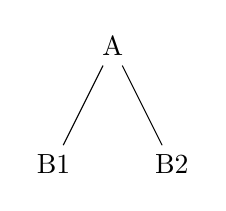
\begin{tikzpicture}
\node {A}
child{node {B1}}
child{node {B2}}
;
\end{tikzpicture}
\end{Verbatim}
      \end{minipage} gives  \hspace{1cm}
      \begin{minipage}{.20\linewidth}
        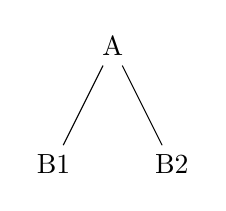
\begin{tikzpicture}
          \node {A}
            child{node {B1}}
            child{node {B2}}
          ;
        \end{tikzpicture}
      \end{minipage}
    \item Grids: use \verb|\draw[<options>] (a) grid (b)| where \texttt{(a)} and \texttt{(b)} are the endpoint of a diagonal (we assume a rectangular mesh). Options may include \texttt{step=<n>}, which sets the width of the cells. The options \texttt{xstep} and \texttt{ystep} are available, as well.
    \item Arrows - heads: \href{https://gist.github.com/AndiH/f99d9b0cbd3519c27af5b96cfbeff97c}{list}, customization \href{https://tex.stackexchange.com/questions/5461/is-it-possible-to-change-the-size-of-an-arrowhead-in-tikz-pgf/161238#161238}{here}.
    \item One may want to have a look at the section about loops, \autoref{sec:loops}.
    \item ATTENTION: for big pictures it is advised to used the \texttt{TikZ} library \texttt{external} in order to avoid regenerating the picture ad each compilation. It basically create separates pdf that will be included in the followings compilations.
      \begin{itemize}
        \item You are invited to read the related chapter in the manual (it should be the 87).
        \item \LaTeX{} compilation needs to be called with the \verb|-shell-escape| option: the compiler should be allowed to run commands to build the external figures.
        \item The \texttt{list and make} mode (activated with \verb|\tikzexternalize[mode=list and make]|) will create a list of the external figure. This list can be processed with \texttt{make}, Hence one has to \begin{inparaenum}[(i)] \item compile the pdf, \item run \verb|make -f -j 4 file.makefile|, \item compile the sources again to ensure the external pictures are included\end{inparaenum}. Notice that the \texttt{make} step can be done in parallel (cf.~\verb|-j <n>|).
          \begin{itemize}
            \item Of course the make step will not always be included in the compilations steps of the automatic compiler. Look \href{https://tex.stackexchange.com/questions/145501/integrating-latexmk-and-tikz-external-mode-list-and-make}{here} for an example of integration with \texttt{latexmk} (see \autoref{sec:latexmk}).
          \end{itemize}
        \item Load with \verb|\usetikzlibrary{external}| or (if loaded) \verb|\usepgfplotslibrary{external}|.
        \item Prefix: it can easily become pretty messy, a prefix can be used to store the files in a directory: \verb|\tikzsetexternalprefix{dir_ext/}|.
        \item Enable, the first time use: \verb|\tikzexternalize|. Disable: \verb|\tikzexternaldisable|. After a disabling, re-enable: \verb|\tikzexternalenable|.
        \item Choose the type of check to perform to see a compilation is needed (via \texttt{tikzset}): \verb|external/up to date check=<type>|: \texttt{simple} (default, just existence), \texttt{md5}, \texttt{diff}.
        \item Force remake of the figure (via \texttt{tikzset}): \verb!external/force remake=true|false!, or just the following picture  \verb!external/remake next=true|false!.
        \item Choose figure name (the one used in the generated pdf): \verb|\tikzsetfigurename{<name>}|, \verb|\tikzsetnextfilename{<name>}|.
        \item \verb|external/only named|: only figures which have be given a name (cf.~here above) are externalized.
        \item Warnings may be issued when using externalization and compiling with draft mode activated. Since the figures are now external pdf they are skipped accordingly to the draft mode. However, the dimensions of the placeholders are not the right one. The solution is \href{https://tex.stackexchange.com/a/82224/206129}{here}:
\begin{verbatim}
\pgfkeys{/pgf/images/include external/.code=\includegraphics{#1}}
\end{verbatim}
      \end{itemize}
%
  \end{itemize}
  %%%%%%%%%%%%%%%%%%%%%% pgfplots
  \subsection{\texttt{pgf(plots)}}
  \label{sub:pgfplots}
  With an \emph{abuse of notations}, here we gather both \texttt{pgf} and \texttt{pgfplots} (and related) tricks. Here is the \href{http://ctan.tetaneutral.net/graphics/pgf/contrib/pgfplots/doc/pgfplots.pdf}{manual}.

  Before going into the details, if you are familiar with \texttt{gnuplot} you may want to check the package \href{http://mirror.ibcp.fr/pub/CTAN/macros/latex/contrib/gnuplottex/gnuplottex.pdf}{\texttt{gnuplottex}} out.

  \begin{itemize}
    \item Basic math operations: compute the result of an expression \verb|\pgfmathparse{<expr>}|, retrieve it with \verb|\pgfmathresult| and use it. It is advised to store it in a variable with \verb|\pgfmathsetmacro\newmacro{\cmd}|
\begin{verbatim}
  \pgfmathparse{sqrt(4)*6}
  \pgfmathsetmacro\result{\pgfmathresult}
\end{verbatim}
    \item Basic plotting: examples in \href{run:./ex_plot.tex}{\texttt{ex\_plot.tex}} (preview \href{run:./ex_plot.pdf}{here}).
    \item 3D plot: \verb|\addplot3| example in \href{run:./ex_plot.tex}{\texttt{ex\_plot.tex}}
      \begin{itemize}
        \item For surface plots, use option \verb|surf| or \verb|mesh|. Watch out for the matrix-like structure that your data must have in order to be interpreted as an actual surface. In particular, blank-lines are very important and separate two rows.
      \end{itemize}
    \item Define commands, set global options: \verb|\pgfplotsset{[...]}|, usually in preamble (advice: use \verb|\pgfplotsst{compt=newest}| for compatibility with the most recent available version).
    \item External plot shape: The plot is usually square, one may prefer to stretch it, here are some options
      \begin{itemize}
        \item \verb!x|y post scale=<n>!;
        \item \verb!x|y scale=<n>!;
        \item \verb|unit vector ratio=<x_value> <y_value>| e.g.~\verb|unit vector ratio=2 1| for a \texttt{x} axis two times longer than the \texttt{y} one
      \end{itemize}
    \item Change the width: \texttt{width=<n>cm}.
    \item Lines\ldots
      \begin{itemize}
        \item Styles: \texttt{solid}, \texttt{dashed}, \texttt{dotted}, \texttt{dashdotted}, \texttt{dashdotdotted}; two modifiers can be use in combination with the styles: \texttt{densely}, \texttt{loosely} (e.g.~\texttt{densely dotted}, \texttt{loosely dashed}).
        \item Width: \texttt{ultra thin}, \texttt{very thin}, \texttt{thin}, \texttt{semithick}, \texttt{thick}, \texttt{very thick}, \texttt{ultra thick}. Or just: \verb|draw[line width=<n>cm, <...>] <...>;|
        \item {\bfseries ATTENTION:} the styles are passed to the markers as well, hence the markers may not appear well printed. When using \texttt{dashed, dotted} or similar remember to add also \verb|mark options={solid[,...]}|, or also \verb|every mark/.append style={solid}| (possibly in a global setting).
      \end{itemize}
    \item Markers\ldots
      \begin{itemize}
        \item \texttt{only marks} vs. \texttt{no markers}.
        \item \texttt{mark repeat=<n>}, filter the markers, print only every \texttt{n}.
        \item Look here above at the line style items in order to prevent weird looking markers.
        \item Use markers outside \texttt{TikZ} environments: \verb|\pgfuseplotmark{<marker_code>}|; e.g.~\verb|\pgfuseplotmark{square*}| (a \verb|\raisebox{<how_much>}{<what>}| may be needed). However, use \verb|\label{<label>}| and \verb|\ref{<ref>}| when possible.
      \end{itemize}
    \item \verb|draw=none|: (actually a \verb|TikZ| key) "switches off" line and marker drawing
    \item Plot style\ldots
      \begin{itemize}
        \item Smoothing a plot: \verb|\addplot[smooth[,...]]|
        \item Constant (stairs) plot: options \texttt{const}/\texttt{jump plot} and you may want to choose the position of the mark (\texttt{const plot mark mid}/\texttt{right}/\texttt{leftt}) and fill (\texttt{fill=<color>}). Try also \texttt{jump plot}.
        \item \texttt{clip mode=individual}: later plots are plotted on top of preceding markers, otherwise markers are plotted in a second phase and they always overwrite any lines (the order doesn't matter). Hence, with \texttt{individual} a line and its markers are always on the same layer, and if a line covers another one, the latter's markers are covered as well.
      \end{itemize}
    \item Legend\ldots
      \begin{itemize}
        \item Have a look at \verb|legend to name=<name>|, which, combined with \verb|\ref{<name>}| allows one to draw a complete legend even outside a \texttt{tikz} scope.
        \item Exclude plot from legend (and cycles): option \verb|forget plot|.
        \item Transparency: the legend box has by default a solid white background, hence it covers part of the canvas. E.g.
\begin{verbatim}
legend style={fill=none} % see-through
legend style={fill=white,fill opacity=0.3,draw opacity=1,%
              text opacity=1} % Custom
\end{verbatim}
        \item Font size: \verb|legend style={font={\scriptsize}}|
        \item Legend box color: \verb|legend style={draw={<color>}}| or \verb|none| for no box.
        \item Alignment: \verb!legend cell align=left|center|right!
        \item Scale: \verb|legend style={nodes={scale=0.7}}|
        \item Legend outside the plot: add \texttt{legend pos=outer north east} (only \texttt{north east} is available so far); or specify the position: \verb|legend style={at={(0.5,-0.1)},anchor=north}|, mind that the coordinates are relative to the axis line, hence those mean below the chart in the middle.
        \item More columns / horizontal growing: \verb|legend style={legend columns=<n>}| where \texttt{n} is the wished number of columns, \texttt{-1} means \emph{horizontally}. For horizontal, one can also use \texttt{transpose legend}
        \item Add lines not related to plot: first, use \verb|\addlegendimage{empty legend}|, the use \verb|\addlegendentry{<lorem>}| to fill the newly line. This could be useful for giving the legend a title. Of course the order is important.
        \item Interesting options: \texttt{reverse legend} (invert the order), \texttt{draw=none} (no legend bow)
      \end{itemize}
    \item Cycle lists. When printing more than one plot on the same canvas, if no options are given \texttt{pgfplots} will choose a line style itself in order to identify easily the plots. Those are the \texttt{cycle list}s.
      \begin{itemize}
        \item Choose the list to use by passing option \verb|cycle list name=<name>| or define directly one via \verb|cycle list|
        \item Some preloaded cycle lists are: \texttt{color}, \texttt{black white}, \texttt{mark list} (and starred version), \texttt{color list} (and starred version), \texttt{linestyles} (and starred version). Ed: I personally like the \texttt{exotic}, it reminds me of what you get on the newest \texttt{Matlab} or \texttt{pyplot}.
        \item Define new lists
\begin{verbatim}
\pgfplotscreateplotcyclelist{ACMilan}{%
  {color=red,solid},
  {color=black,solid},
  {color=red,dashed},
  {color=black,dashed} % <- No comma on the last
}
\end{verbatim}
        \item MIND:
          \begin{itemize}
            \item \verb|\addplot [<opt>]|: the style is entirely defined by \verb|<opt>| and \verb|<opt>| only,
            \item \verb|\addplot+[<opt>]|: \verb|<opt>| is appended to the \texttt{cycle list} option.
          \end{itemize}
      \end{itemize}
    \item Grouping plots: if you have to print plots side-by-side, many options are available: using \verb|subfigure| (see \fullref{sec:Floats}), only one \texttt{figure} and only one \texttt{tikzpicture} multiples \texttt{axis},\ldots{} A simple way might be to use the utility proposed by library \texttt{groupplots}. Use environment \verb|groupplot|, examples below and also in \href{run:./ex_plot.tex}{\texttt{ex\_plot.tex}}.
\begin{verbatim}
\usepgfplotslibrary{groupplots}
\begin{tikzpicture}
  \begin{groupplot}[%
    group style={%
      group size=2 by 1,
    },
    % The following applies to every subplot
    width=0.48\linewidth,
    ]
    \nextgroupplot
      % Now use addplot as you would do normally
      \addplot[blue] table[x index=0,y index=1] {tab1.dat};
    \nextgroupplot
      \addplot[blue] table[x index=0,y index=2] {tab1.dat};
  \end{groupplot}
\end{tikzpicture}
\end{verbatim}
      \begin{itemize}
        \item No \texttt{axis} environment is needed
        \item Command \verb|\nextgroupplot| indicates switching the following plot
          \begin{itemize}
            \item Order: From top to bottom, from right to left
            \item Pass option \verb|\nextgroupplot[group/empty plot]| to skip the following position
          \end{itemize}
      \end{itemize}
    \item By default, \texttt{pgfplots} leaves some withespace between the axes/plot side and the outermost point of the plot. You might control the behaviour by setting the \texttt{enlarge limits} parameter
\begin{verbatim}
enlarge x limits=auto|true|false|upper|lower|<val>|value=<val>
% or even...
enlarge x limits=abs value=<val>|abs=<val>|rel=<val>
\end{verbatim}
      You may replace \texttt{x} with the concerned component or use \texttt{enlargelimits=} for all the components at the same time
    \item Error \texttt{Dimension too large}: look \href{https://tex.stackexchange.com/questions/13816/dimension-too-large-while-plotting-with-pgfplots}{here}, use
\begin{verbatim}
restrict y to domain:<min>:<max>
\end{verbatim}
      Mind however that this filter somehow the points bu does not set the limits of the plot, hence you might want to set also e.g.~\texttt{ymin=<min>}
    \item Show colorbar: option \texttt{colorbar}. Yup, that was easy. Default is vertical on the right. One may choose \texttt{colorbar left}, \texttt{colorbar horizontal}.
    \item Ticks: ticks are the markers on the axes. They are computed automatically but you can force them
      \begin{itemize}
        \item \texttt{xtick distance}: set the distance between two ticks. The version \texttt{ytick} is available as well.
        \item \texttt{xtick={1,2,2.1,2.2}}: choose where to draw them. The version \texttt{ytick} is available as well. Only the selected ticks are marked, that is not an add (for addition, see below). Instead of the list, you can pass \texttt{empty} or \texttt{data} (all and only coordinate of the plot).
        \item \texttt{xticklabel={1e0,Marco,2}}: choose what is printed. The version \texttt{ytick} is available as well. Set the style with \texttt{xticklabel style}.
        \item \texttt{extra x ticks}: additional ticks. Control with \texttt{extra x tick labels} and \texttt{extra x tick style}. The version \texttt{y tick} is available as well.
      \end{itemize}
    \item Help grids:
      \begin{itemize}
        \item Set the level of the help grid that should appear on your plot via the option \verb|grid=<type>|. Possible types are \verb|none|, \verb|major|, \verb|minor|, \verb|both|
        \item Set the style of a type of grid: e.g.~\verb|major grid style={dotted,very thin}|
        \item Even if the \verb|minor| (or \verb|both|) is requested, it may not actually printed. In fact, in order to be printed the plot need to have minor ticks as well. For instance, use \verb|minor tick num=<n>| where \verb|n| is how many minor ticks between two major one you want.
      \end{itemize}
    \item \verb|forget plot|: it has already been mentioned that this allows to skip a plot from a legend. Additionally, the "forgotten" plots, will not affect the axis of the plot, been considered in the \texttt{cycle}s, not increase the number of plots.
    \item Print zero axes: have a look \href{https://tex.stackexchange.com/questions/55718/how-can-i-add-a-zero-line-to-a-plot}{here}.
    \item A couple of ideas about confidence levels and errors: one is \href{https://tex.stackexchange.com/questions/185111/adding-confidence-intervals-in-pgfplots}{here} and the other \href{https://tex.stackexchange.com/questions/96954/plotting-two-time-series-with-bounds}{there}.
    \item Fill area between two lines: \href{http://pgfplots.net/tikz/examples/fill-between-plots/}{here} is a really cool example.
    \item Idea: \texttt{clickable coords} make something (dis)appear at mouse click.
    \item ATTENTION: for big pictures it is advised to used the \texttt{TikZ} library \texttt{external} in order to avoid regenerating the picture ad each compilation.
    \begin{itemize}
      \item A remark about compiling time when plotting from an external file is in the following, \verb|pgfplotstable|-related section.
    \end{itemize}
    \item \texttt{tikz} and \texttt{beamer} overlays
      \begin{itemize}
        \item Out of the box, only the overlay \texttt{only} works with \verb|\addplot|.
        \item Some convenient definitions are given in the library \verb|\usetikzlibrary{overlay-beamer-styles}|, part of the \href{https://mirrors.chevalier.io/CTAN/graphics/pgf/contrib/aobs-tikz/aobs-tikz.pdf}{\texttt{aobs-tikz}} package. An \href{https://tex.stackexchange.com/questions/175228/how-can-i-make-beamer-overlays-with-tikz-node-attributes}{example}.
      \end{itemize}
  \end{itemize}

\subsubsection{\texttt{pgfplotstable}}
\label{ssub:pgfplotstable}
\texttt{pgfplotstable} is a useful sub-package of \texttt{pgfplots} which, for example, enables you to read and plot directly data from a file if \href{http://mirrors.standaloneinstaller.com/ctan/graphics/pgf/contrib/pgfplots/doc/pgfplotstable.pdf}{\texttt{pgfplotstable}}.

In what follows, \verb|<table>| can be either the file to be read, or a macro associated to an already read table, or a hardcoded table (cf.~\href{run:./ex_plot.tex}{\texttt{ex\_plot.tex}}).

Two are the main reasons to use (and to love) \texttt{pgfplotstable}: creating plots from data using \verb|\addplot table {<table>}|, typesetting tables with \verb|\pgfplotstabletypeset{<table>}| (mind that this is a just an interface and \texttt{pgfplotstable} will only print the content in a format compatible with a \texttt{tabular} or alike environment). Examples are in \href{run:./ex_plot.tex}{\texttt{ex\_plot.tex}}.

  \begin{itemize}
    \item Global settings / style definitions: e.g.~\verb|\pgfplotstableset{[...]}|
    \item \texttt{pgfplotstable} works column-wise. Need to work by rows?
      Use (\href{https://tex.stackexchange.com/questions/183519/plotting-data-from-rows-instead-of-columns-in-latex}{here})
\begin{verbatim}
  \pgfplotstabletranspose\newtable{<table>}
\end{verbatim}
    \item Separators: options \verb|col sep=<char>,row sep=<char>|, the default are white-space and newline. For \texttt{csv}, use \verb|col sep=comma|.
    \item Ignore characters: option \verb|ignore chars=<chars>|.
    \item \verb|clear infinite|: if NaN or infinite are found, they are considered as empty cells.
    \item Bad data: select how to treat bad data: e.g.~\verb!unbounded coords=jump|discard!.
    \item How to treat empty cells: \verb|empty cells with={<...>}|.
    \item Option \verb!header=true|false|has colnames!. Tell whether or not the first non-commented line should be treated as the names of the columns. \texttt{has colnames} force it even if it is number and not string.
    \item Sort\&Filter: options \verb|sort,sort key={<key>}| and also \href{https://tex.stackexchange.com/questions/66177/how-can-i-filter-select-data-from-a-table-and-plot-it}{here}.
    \item Warnings: when filtering or discarding data, one gets warnings, shush them with \texttt{filter discard warning=false}.
    \item Get cell content: For current row (replace \verb|this| with \verb|prev| for previous row or with \verb|next| for next row)
      \begin{itemize}
        \item \verb|\thisrow{<col_name>}|: get the value and use it now.
        \item \verb|\thisrow{<col_name>}{<\macro>}|: get the value and store it in the macro.
        \item If one wants to use column indexes (instead of column names): e.g.~\verb|\thisrowno{<n>}| (zero-based) (\verb|\thisrow{[index]<n>}| should work too).
        \item \verb|\pgfplotstablegetelem{<row>}{<col>}\of{<table>}|. The second argument must be a column name, if one wishes to use an index replace it with: \verb|{[index]<n>}|.
        \item \verb|\pgfplotstablegetcolumnnamebyindex{0}\of{\mytab}\to{\firstcolumn}|
      \end{itemize}
    \item Create columns: two main ways
      \begin{itemize}
        \item Online: dedicated option, the column is used directly
\begin{verbatim}
\pgfplotstabletypeset[%
  create on use/newcol/.style={create col/.<type>={[...]}]{<table>}
\end{verbatim}
        It works both with \verb|\pgfplotstabletypeset| and \verb|\addplot table|
        \item Offline: dedicated command, the columns will be added to the table and usable elsewhere
\begin{verbatim}
\pgfplotstablecreatecol{create col/.<type>={[...]}}{<table>}
\end{verbatim}
        \item Mind that if you want to perform operation on created columns (e.g.~summing two new columns), the columns must be created offline (\href{run:./ex_plot.tex}{\texttt{ex\_plot.tex}}).
      \end{itemize}
    \item Ideas on columns management: \href{https://tex.stackexchange.com/questions/79150/pgfplotstable-how-to-access-column-name}{here}.
    \item Vertically concatenate two tables (only common columns are printed, only one header is printed): \verb|\pgfplotstablevertcat{\mytabone}{mytabtwo}|, then merged is stored in \verb|\mytabone|, hence print it: \verb|\pgfplotstabletypeset{\mytabone}| (\href{https://tex.stackexchange.com/questions/19877/add-rows-to-a-pgftable}{here}).
    \item Modify row \texttt{<n>}: e.g.~print line before row number 4
\begin{verbatim}
\pgfplotstableset{%
  every row no 4/.style={before row={\hrule}}}
\end{verbatim}
    \item Compiling performances: reading at each time vs. \verb|\pgfplotstableread|. It may happen that one has a big (many columns and/or many rows) file to plot, possibly it should be used several times. If you are a not-too-bad developer, you'd be lead to read it once, store it in a variable and reuse it again and again, like this
\begin{Verbatim}[samepage=true]
\pgfplotstableread{file.dat}\mytable
% Repeat several times
% [...]
\addplot table {\mytable};
\end{Verbatim}
  However, as it is explained \href{https://tex.stackexchange.com/a/304734/206129}{here}, a faster solution is
\begin{Verbatim}[samepage=true]
% Repeat several times
% [...]
\addplot table {file.dat};
\end{Verbatim}
  For big files, the speed-up might be 2 (I indeed observed it) and more!
    \begin{itemize}
      \item Be also aware of \href{https://tex.stackexchange.com/questions/236398/speed-up-plotting-data-with-many-columns}{this}.
      \item For plots with a lot of data-points, using option \verb|each nth point=<n>| (\href{https://tex.stackexchange.com/a/68658/206129}{here}) may be worth it. If you think that reducing drastically your data points may deteriorate the quality of your plot, try adding option \verb|smooth|, too.
    \end{itemize}
  \end{itemize}

%%%%%%%%%%%%%%%%%%%%%%%%%%%%%%%%%%%%%%%%%%%%%%%%%%%%%%%%%%%%%%%%%%%%%%%%%%%%%%%%
%%%                   SECTION: DRAFT
%%%%%%%%%%%%%%%%%%%%%%%%%%%%%%%%%%%%%%%%%%%%%%%%%%%%%%%%%%%%%%%%%%%%%%%%%%%%%%%%
\section{Draft}
\label{sec:Draft}
Writing a document can be not so easy by itself, and we think that writing it with \LaTeX{} should not make it harder. A couple of trick are given here below for example to compile in an approximated (no images, no hyperlinks,\ldots) but faster way, to help you with the layout, or with keeping track of the labels.

\begin{itemize}
  \item The \verb|draft| option (passing it to the \verb|article| class, for example) will make visible the lines where you're exceeding the margin (little black vertical bar at the end of the line) and it will not load the figures but only reserve a place on the page (at least, you can see the layout): the compilation is faster
\begin{verbatim}
\documentclass[draft]{article}
\end{verbatim}
    \begin{itemize}
      \item You can avoid including a single picture by passing \texttt{draft} option:
\begin{verbatim}
\includegraphics[draft]{hidden_picture}
\end{verbatim}
      \item With more recent versions of \LaTeX{} a place-holder figure named \texttt{example-image-a} is available: \verb|\includegraphics[scale=0.6]{example-image-a}|
      \item Another way for having place-holder pictures is via the package \texttt{todonote} (see below) and its command
\begin{verbatim}
\missingfigure{A description of the future figure}
\end{verbatim}
    \end{itemize}
  \item Show all labels that you have set in pdf (useful when writing the source and you don't want to scroll to know the exact name that you chose for the equation you want to refer to): package \href{http://ctan.mines-albi.fr/macros/latex/contrib/showlabels/showlabels.pdf}{\texttt{showlabels}}.
  \begin{itemize}
    \item ATTENTION: make sure you load it after \texttt{amsmath} and alike, and after \texttt{hyperref}.
    \item Add support for a command: example
\begin{verbatim}
\showlabels{bibitem}
\showlabels{cite}
\end{verbatim}
  \end{itemize}
  \item An alternative for printing out the labels is \href{http://ctan.tetaneutral.net/macros/latex/required/tools/showkeys.pdf}{\texttt{showkeys}}.
  \item Fancy and colorful todo notes from the \href{http://tug.ctan.org/macros/latex/contrib/todonotes/todonotes.pdf}{\texttt{todonotes}} package.
  \item With \texttt{beamer}: \autoref{sec:Beamer}.
  % % Let the following be the last
  \item It could be interesting to define a command that may be set to either \texttt{draft} or \texttt{final}. Pass this command to all the packages listed just here above, hence you just need to modify this macro in order to change the setting of all the packages. Mind that it goes before the class:
\begin{verbatim}
\providecommand{\DraftOrNot}%
%{draft}
{final}
\documentclass[\DraftOrNot]{article}
\end{verbatim}
    Another possibility is to load the package \href{https://ctan.crest.fr/tex-archive/macros/latex/contrib/oberdiek/ifdraft.pdf}{\texttt{ifdraft}} which detects if the \texttt{draft} option is activated and create a boolean accordingly, so that one can use \verb|\ifdraft{...}{...}|
  \item One may want to check the part about the large comments out: \fullref{sec:Miscellaneous}.
\end{itemize}

This goes beyond the scope of the section and of the document too, but something that you should be aware of when editing a \LaTeX{} file is forward- and backward-search. In a nutshell, this is like, I'd say, having a link between the file editor and the pdf viewer, so that, for instance, with some manipulation you select a word in the editor and the viewer pops up at the selected spot, or vice versa. Think about you finding a typo while proofreading a document of several pages, you click on it and the editors goes directly to it, without you browsing around. That could save time. Most of IDE specialized on \LaTeX{} (see for instance \fullref{sec:texmaker}) have it, if you are used to more basic editor, you should do some tweaking around, but usually solutions are available.

%%%%%%%%%%%%%%%%%%%%%%%%%%%%%%%%%%%%%%%%%%%%%%%%%%%%%%%%%%%%%%%%%%%%%%%%%%%%%%%%
%%%                   SECTION: REFERENCING & HYPERLINKS
%%%%%%%%%%%%%%%%%%%%%%%%%%%%%%%%%%%%%%%%%%%%%%%%%%%%%%%%%%%%%%%%%%%%%%%%%%%%%%%%
\section{Referencing \& Hyperlinks}
\label{sec:Referencing}
\begin{itemize}
  \item It is a good habit to follow this structure when naming a \texttt{label}: \verb|\label{type:desc}|. \texttt{type} is short for the type of element that is being named, for instance \texttt{fig} for a figure/picture, \texttt{sec} for a section, \texttt{eq} for an equation and so on. \texttt{desc} should clearly identify the element. For instance, see what was done wit the Euler equation in \fullref{sec:math}: \verb|\label{eq:euler}|.
  \item Some tips already given in \fullref{sec:math} and \fullref{sec:Items}
  \item Mind the tricky behavior of label with overlays in \texttt{beamer} (\autoref{sec:Beamer}).
  \item Useful packages for referencing: \href{ftp://tug.ctan.org/pub/tex-archive/macros/latex/contrib/hyperref/doc/manual.pdf}{\texttt{hyperref}} and \href{http://ctan.mines-albi.fr/macros/latex/contrib/cleveref/cleveref.pdf}{\texttt{cleveref}}. It is possible to load both of them at the same time with a little precaution:
\begin{verbatim}
\usepackage{hyperref} % ATTENTION: to be loaded AFTER math related packages
\usepackage[noabbrev]{cleveref} % ATTENTION: to be loaded AFTER hyperref
\end{verbatim}
  \item ATTENTION: \texttt{cleveref} does not produce hyperlinks, it is just a smart reference-management tool. This option is provided only by \texttt{hyperref}.
  \item Referencing with type (that is, automatically getting \emph{section 1.1})
\begin{verbatim}
\autoref{label} % with package hyperref
\cref{label}    % with package cleveref
\end{verbatim}
  \begin{itemize}
    \item Define names for user-defined environments
\begin{verbatim}
\newcommand{\<env>autoref}{<printedenvname>} % with package hyperref
\crefname{<env>}{<singular>}{<plural>} % For cref (cleveref)
\end{verbatim}
    \item Capitalize the name (e.g.~\emph{Section 1.1}): possible with \texttt{cleveref}
\begin{verbatim}
\Cref{label} % instead of cref
\end{verbatim}
          or globally
\begin{verbatim}
\usepackage[capitalise]{cleveref} % both \cref and \Cref capitalized
\end{verbatim}
  \end{itemize}
\item Referencing by names (and not numbers): have a look \href{https://texfaq.org/FAQ-nameref}{here}. Other tips below in \texttt{hyperref}.
\end{itemize}

The \texttt{hyperref} package enables to create hyperlinks. Here is an \href{https://www.overleaf.com/learn/latex/hyperlinks}{overview} (the previous word is indeed a hyperlink! Click on it!). The basic command is \verb|\href{<link_address>}{<place_holder>}|: \verb|place_holder| is what is printed in the document and \verb|link_address| is the actual address.
\begin{itemize}
  \item Webpages: it is better to prepend \texttt{http://} (or indeed \texttt{https://}) to the link in order not to have weird behavior, e.g.~\verb|https://www.edf.fr|.
  \item Email address: prepend \texttt{mailto:} to the address, e.g.~\verb|\href{mailto:jbl_pdg@gmail.com}{JBL}|.
  \item Local file: prepend \texttt{run:} to the file you want to open, e.g.~\verb|\href{run:/path/to/tips.pdf}{tips}|.
  \item Option \verb|linktoc=<type>| let you choose if the section name (\texttt{section}, default), page number (\texttt{page}), both (\texttt{all}) or none (\texttt{none}) link to the section.
  \item Create additional bookmarks: \verb|\pdfbookmark[<level>]{<title>}{<label>}|. \texttt{level} is a number, \texttt{0} corresponds to chapter.
  \item \verb|\nameref| reference by name and not by number. If you want to put everything together (number \emph{and} name), have a look \href{https://tex.stackexchange.com/a/121871/206129}{here}.
\end{itemize}

Some tips about \texttt{cleveref}:
\begin{itemize}
  \item \verb|\labelcref{<label>}|: print only the label. E.g.~\texttt{1.1} (without \texttt{Section}).
  \item \verb|\namecref{<label>}|: print only the name, type. E.g.~\texttt{Section} (without \texttt{1.1}).
  \item \verb|\crefrange{<start_label>}{<end_label>}|: typeset a range of references. For uppercase names \verb|\Crefrange{<start_label>}{<end_label>}|
  \item option \texttt{noabbrev} makes \texttt{cleveref} print full reference name, e.g.~\texttt{equation} instead of \texttt{eq.}
  \item option \texttt{poorman}: you are invited to look at it in the \href{http://ctan.mines-albi.fr/macros/latex/contrib/cleveref/cleveref.pdf}{manual}. Basically, if you have to send your \TeX{} sources to someone that does not use \texttt{cleveref}, you can add this option and \texttt{cleveref} will produce a \texttt{sed} script which, once run, will replace all calls to its macros although leaving the output unchanged.
\end{itemize}

%%%%%%%%%%%%%%%%%%%%%%%%%%%%%%%%%%%%%%%%%%%%%%%%%%%%%%%%%%%%%%%%%%%%%%%%%%%%%%%%
%%%                   SECTION: BIBLIOGRAPHY
%%%%%%%%%%%%%%%%%%%%%%%%%%%%%%%%%%%%%%%%%%%%%%%%%%%%%%%%%%%%%%%%%%%%%%%%%%%%%%%%
\section{Bibliography}
\label{sec:Bibliography}
\begin{itemize}
  \item \href{https://www.overleaf.com/learn/latex/Bibliography_management_with_bibtex}{Here} you can find a basic introduction to the bibliography in \LaTeX. A good habit is to create a separate \texttt{.bib} file. Some pdf managing programs (such as \href{https://www.zotero.org/}{Mendeley} or \href{https://www.zotero.org/}{Zotero}) automatically build the \texttt{.bib} file for you, with all the pdf in your library.  \item There are several ways to manage the bibliography in \TeX{} files: \texttt{biblatex}, \texttt{natbib},\ldots
  \item Examples of bibliography styles can be found \href{https://www.overleaf.com/learn/latex/Bibtex_bibliography_styles}{here};
  \item Print references even if they were not cited: \verb|\nocite{<ref_name>}|. Print all the references: \verb|\nocite{*}|.
  \item Change the name of the bibliography title: redefine \verb|\refname| or \verb|\bibname| (it depends on the package you are using). Ex
\begin{verbatim}
\renewcommand{\refname}{Main References}
\end{verbatim}
  \item Change the spacing between title and first item: use (mind: it can be used in the preamble only) \verb|\AtBeginBibliography{\vspace*{-2cm}}|
    \begin{itemize}
      \item One can actually replace the spacing with anything he/she wants to run at the beginning.
    \end{itemize}
  \item Sometimes the order of the citations is not the right one or what you wish. For instance, if alphabetical order is requested, sometimes only the first authors are considered. You can fix/force the order with \verb|\noopsort{<label>}|. \texttt{label} will not be printed but it will be considered when defining the order. Some details are \href{http://www.texfaq.org/FAQ-bibprefixsort}{here}. See also this \href{https://tex.stackexchange.com/a/298531/206129}{answer} and the related question. Add in the \texttt{.bib} file
\begin{verbatim}
@preamble{ "\providecommand\noopsort[1]{}" }
@article{ABC14,
 author  = {Anna \noopsort{1}Abel and Betty Boom and Chris Conway},
 journal = {Journal 1}, title = {Title 1}, year = {2014},
}
@article{AD10,
  author  = {Anna \noopsort{2}Abel and Deirdre Donald},
  journal = {Journal 2}, title = {Title 2}, year = {2010},
}\end{verbatim}
    You can try different locations where to put \verb|\noopsort{}|. For instance, after the first author name, in the year or title fields. Remember however, that if you put it with the author name, you should use it in every entry with the same author.
\end{itemize}

  \subsection{\texttt{natbib}}
  \label{sub:natbib}
  \href{https://ctan.crest.fr/tex-archive/macros/latex/contrib/natbib/natbib.pdf}{User guide} (in \href{http://mirror.ibcp.fr/pub/CTAN/info/translations/natbib/fr/f-natbib.pdf}{French} too!) and \href{http://mirror.ibcp.fr/pub/CTAN/macros/latex/contrib/natbib/natnotes.pdf}{cheat-sheet} or this \href{http://merkel.texture.rocks/Latex/natbib.php}{cheat-sheet too}. If you do not use a \LaTeX{} integrated editor (IDE) (although it could be useful to know this anyway) but compile from terminal, you should:
    \begin{enumerate}
      \item Compile one time with your preferred compiler (e.g.~\texttt{pdflatex}: \verb|$pdflatex main.tex|);
      \item Compile the bibliography with \texttt{bibtex}: \verb|$bibtex main.aux|;
      \item Re-compile \textbf{twice} your \texttt{.tex} in order to have all the references linked and working.
    \end{enumerate}

    \begin{itemize}
      \item If you have more than one bibliography files, just put them in the \texttt{bibliography} command separated by a comma (remember that you should not write the extension \texttt{.bib}):
    \begin{verbatim}
      \bibliography{my_biblio_1,my_biblio_2}
    \end{verbatim}
      \item \texttt{natbib} automatically creates a new section for the references. One get rid of it by overriding the \texttt{bibsection} command: one may choose to defining it as a subsection, or simply remove it, as follows
\begin{verbatim}
  \renewcommand{\bibsection}{}
\end{verbatim}
      \item For three or more authors, \texttt{natbib} will print \emph{First\_Author et al.}. In order to print all the authors, use the starred-version of the commands: \verb|\citep*{<ref_name>}|
      \item Multiple bibliography / bibliography in each chapter: package \href{http://wiki.davidhaberthuer.ch/latex#chapterbib}{\texttt{chapterbib}} and option \texttt{sectionbib} as explained \href{http://wiki.davidhaberthuer.ch/latex#chapterbib}{here} or \href{https://tex.stackexchange.com/questions/229846/different-bibliographies-for-each-chapter-with-shared-references}{here}. Remember to call \verb|\bibliography{<chap_bib>}| in each chapter. Another possibility is package \href{http://mirrors.standaloneinstaller.com/ctan/macros/latex/contrib/bibunits/bibunits.pdf}{\texttt{bibunits}}, have a look \href{https://texfaq.org/FAQ-chapbib}{here}.
      \item ATTENTION: It does not work well with \texttt{beamer} (\autoref{sec:Beamer}).
    \end{itemize}

  \subsection{\texttt{biblatex}}
  \label{sub:biblatex}
  \href{http://mirror.ibcp.fr/pub/CTAN/macros/latex/contrib/biblatex/doc/biblatex.pdf}{User guide} (in the introduction, there is a nice overview of other bibliography-related packages which could be useful). A quick \href{https://www.overleaf.com/learn/latex/Articles/Getting_started_with_BibLaTeX}{tutorial} (see also \href{https://www.overleaf.com/learn/latex/Biblatex_citation_styles}{this} and \href{https://www.overleaf.com/learn/latex/Biblatex_bibliography_styles}{that} for examples of citation/bibliography styles). And a useful \href{http://tug.ctan.org/info/biblatex-cheatsheet/biblatex-cheatsheet.pdf}{cheatsheet}. \texttt{biblatex} relies on \texttt{biber}, thus the compiling sequence becomes:
    \begin{enumerate}
      \item Compile one time with your preferred compiler (e.g.~\texttt{pdflatex}: \verb|$pdflatex main.tex|);
      \item Compile the bibliography with \texttt{biber}: \verb|$biber main.bcf|;
      \item Re-compile \textbf{twice} your \texttt{.tex} in order to have all the references linked and working.
    \end{enumerate}
  If you use an IDE, you may have to change the compiling stage command to something like: \verb|biber %.bcf|. However, \texttt{biber} is not available on the EDF-controlled OS, but you can change the bibliography compiler. When loading \texttt{biblatex} use \texttt{bibtex} or \texttt{bibtex8} as backend (both available on EDF PCs): e.g.~\verb|\usepackage[backend=bibtex]{biblatex}|. Now the compiling process will be the same as for \texttt{natbib}:
    \begin{enumerate}
      \item Compile one time with your preferred compiler (e.g.~\texttt{pdflatex}: \verb|$pdflatex main.tex|);
      \item Compile the bibliography with \texttt{bibtex}, \verb|$bibtex main.aux|, or with \texttt{bibtex8}, \verb|$bibtex8 main.aux|;
      \item Re-compile \textbf{twice} your \texttt{.tex} in order to have all the references linked and working.
    \end{enumerate}
    In IDE such as \TeX Maker, the default compiling command is usually \texttt{bibtex}, hence if you are using \texttt{bibtex8} you should modify it accordingly: \verb|bibtex8 %.aux|

  \begin{itemize}
    \item It is preferable to load \texttt{biblatex} \emph{before} \texttt{hyperref};
    \item The file containing the bibliography is set in the preamble, it is advised to do it just after you load the package:
\begin{verbatim}
  \usepackage{biblatex}
  \addbibresource{my_biblio.bib}
\end{verbatim}
    \item Print the bibliography: \verb|\printbibliography|;
    \item Set the style: use option
      \begin{itemize}
        \item \texttt{citestyle=<style>} for the \emph{citation} style (what appears when your call \verb|\cite{}|),
        \item \texttt{bibstyle=<style>} for the style in the list,
        \item \texttt{style=<style>} for setting both of the above.
      \end{itemize}
    \item Sort the citations: \verb|\usepackage[sorting=<style>]{biblatex}|, usually the argument is a combination of \texttt{n} (for name), \texttt{t} (title), \texttt{y} (year) according to the importance (e.g.~\texttt{nyt}, \texttt{nty}).
    \item You can even provide a direct link to your \href{https://www.zotero.org/}{\texttt{Zotero}} bibliography (see the manual).
    \item Footnote-like citation (could be useful in \texttt{beamer}): \verb|\footcite{<ref_name>}|, look also \verb|\footfullcite{<ref_name>}|.
    \item Avoid \emph{et al.}: put in the options when loading the package \texttt{maxnames=<n>} or \texttt{minnames=<n>}.
    \item Suppress "\emph{In:}" in the bibliography: \verb|\renewbibmacro{in:}{}| (\href{https://tex.stackexchange.com/a/10686/206129}{here}).
    \item No URL, ISSN, nor DOI: options \texttt{url=false,doi=false,isbn=false}.
    \item Add \emph{see}, \emph{chapter n} or alike: \verb|\command[<prenote>][<postnote>]{<ref_name>}|. For example, \verb|\parencite[see][chpt 2]{Aliceetal}| gives something like: (see \emph{Alice et al.}, chpt 2)
      \begin{itemize}
        \item If only one optional argument is given, it is understood as post-note. For example, \verb|\parencite[chpt 2]{Aliceetal}| gives (\emph{Alice et al.}, chpt 2).
        \item Using \verb|\cite| with optional arguments inside an optional argument: put the whole command inside curly brackets
\begin{verbatim}
\begin{theorem}[The one and only {\cite[Thm 1]{Aliceetal}}]
  $a^2+b^2=c^2$
\end{theorem}
\end{verbatim}
      \end{itemize}
    \item Citing more than one reference at the same time
      \begin{itemize}
        \item For standard citations, just put a comma-separated list of entries. Capitalized version available.
\begin{verbatim}
\cite{Aliceetal,Bobetal}
\end{verbatim}
        \item For citations with pre- and post-note use \verb|\cites|, which accepts a generic number of arguments. Capitalized version available.
\begin{verbatim}
\cites[see][chpt 2]{Aliceetal}[and][sect 3.1]{Bobetal}
\end{verbatim}
      \end{itemize}
    \item Option \texttt{backref} puts after each bibliography entry the pages/places where that entry has been cited.
    \item Avoid the warning about \texttt{utf8} encoding (possibly if the backend is set to \texttt{bibtex}): pass option \texttt{bibencoding=ascii}. However, this may cause problems if you use non-ASCII character (fancy accented symbols,\ldots).
    \item When using \texttt{biblatex} and \texttt{babel}, it is advised to load \texttt{csquotes} as well, in order to ensure that quoted texts are typeset according to the chosen language rules.
    \item \texttt{giveninits=true}: force initials for given names in bibliography.
    \item Choose the order for given a family name in the bibliography: choose between \texttt{family-given} or \texttt{given-family}. For instance:
\begin{verbatim}
\DeclareNameAlias{sortname}{family-given}
\DeclareNameAlias{author}{family-given}
\DeclareNameAlias{editor}{family-given}
\end{verbatim}
    \item Group of references:
\begin{verbatim}
\DeclareBibliographyCategory{<category}
\addtocategory{<category}{<ref_key>[,<ref_keys>]}
\end{verbatim}
      \begin{itemize}
        \item Print only/other than category: \verb|\printbibliography[[not]category=<category>]|
        \item Print only/other than type: \verb|\printbibliography[[not]type=<type>]|, with \texttt{type} being article, book\ldots
      \end{itemize}
    \item According to the style, the author in the bibliography might be replaced by a dash if it is repeated. One may disable this feature (and always print the author) with the option \texttt{dashed=false} (however, it is available only in the most recent versions ob \texttt{biblatex}: >2016)
    \item In some predefined styles, the mention "\emph{In:}" precedes the article title, for instance. One may remove it by calling: \verb|\renewbibmacro{in:}{}|. Have a look \href{https://tex.stackexchange.com/questions/10682/suppress-in-biblatex}{here} for a custom solution involving only the articles.
    \item ATTENTION: for label printing use \texttt{showkeys} (incompatibility with \texttt{showlabels} and pre/post-cite).
    \item Change size: \verb|\renewcommand{\bibfont}{\scriptsize}|
    \item Multiple bibliography / bibliography in each chapter: take advantage of the \texttt{refsegment} environment as explained \href{https://tex.stackexchange.com/questions/87414/per-chapter-bibliographies-in-biblatex}{here}. You may also want to have a look \href{https://tex.stackovernet.com/fr/q/63260}{here}.
\begin{verbatim}
  \begin{refsegment}
    \chapter{Chpt 1}
    Lorem lipsum
    \printbibliography[segment=1,title={Chpt1 references},heading=subbibintoc]
  \end{refsegment}
  \printbibliography[title={Global references},heading=subbibintoc]
\end{verbatim}
      \begin{itemize}
        \item Remember to change the number of \texttt{segment} according to the chapter
        \item If you plan to use \verb|\include| and \verb|\includeonly| with, for instance, one file per chapter you'd better NOT put \verb|\begin{refsegment}| in the chapter \texttt{.tex} but leave it in the main, in order to avoid problem with undefined segment when \verb|\includeonly| is used
\begin{verbatim}
  \begin{refsegment}
    \include{chpt1}
  \end{refsegment}
  \printbibliography[title={Global references}, heading=subbibintoc]
\end{verbatim}
      \end{itemize}
    \item Warnings may be issued with footnotes and \texttt{beamer} (e.g.~\texttt{Patching footnotes}), although this should happen only in old versions. Have a look at this \href{https://tex.stackexchange.com/questions/202988/beamer-patching-footnotes-warning-patching-footnotes-failed-footnote-detectio}{answer} and this \href{https://tex.stackexchange.com/questions/369266/beamer-and-biblatex-possible-remedy-for-warning-patching-footnotes-failed/405186#405186}{reference} therein.
  \end{itemize}

  Have a look at the \href{http://ctan.mines-albi.fr/macros/latex/contrib/biblatex/doc/biblatex.pdf}{here} for more details about these options/commands and many useful other ones.

%%%%%%%%%%%%%%%%%%%%%%%%%%%%%%%%%%%%%%%%%%%%%%%%%%%%%%%%%%%%%%%%%%%%%%%%%%%%%%%%
%%%                   SECTION: Standalone
%%%%%%%%%%%%%%%%%%%%%%%%%%%%%%%%%%%%%%%%%%%%%%%%%%%%%%%%%%%%%%%%%%%%%%%%%%%%%%%%
\section{\texttt{standalone}}
The standalone bundle allows users to easily place picture environments or other material in own source files and compile these on their own or as part of a main document.  A special standalone class is provided for use with such files, which by default crops the resulting output file to the content. The standalone package enables the user to simply load the standalone files using \verb|\input| inside a main document (from the \href{http://ctan.mines-albi.fr/macros/latex/contrib/standalone/standalone.pdf}{manual}). Basically one can create a file that can be compiled by itself or that can be part or a larger project, without having to change it.
\begin{itemize}
  \item A typical call would be: \verb|\documentclass[border=1mm]{standalone}|.
  \item Packages-related options: \texttt{TikZ}, \texttt{beamer}
  \item Write equations in standalone: use option \texttt{preview}.
  \item Some options:
    \begin{itemize}
      \item \verb|class=<class_name>|: set the underlying layout (article, report\dots)
      \item \verb!crop=true|false!: crop the content to its natural size plus a border
      \item \verb!multi=true|false!: if false only one big page
      \item \verb|multi={<env_name[,...]>}|: create a new page for every \verb|<env_name>| environments
      \item \verb|beamer|: crop is disabled and content shown on a blank \texttt{beamer} frame
      \item \verb|tikz|: load \texttt{TikZ} and set \verb|multi=tikzpicture|
    \end{itemize}
\end{itemize}

\textbf{Remark}: if you just want a minimal layout for a \texttt{documentclass}, an option could also be \texttt{minimal} instead of \texttt{standalone}.

%%%%%%%%%%%%%%%%%%%%%%%%%%%%%%%%%%%%%%%%%%%%%%%%%%%%%%%%%%%%%%%%%%%%%%%%%%%%%%%%
%%%                   SECTION: Thesis
%%%%%%%%%%%%%%%%%%%%%%%%%%%%%%%%%%%%%%%%%%%%%%%%%%%%%%%%%%%%%%%%%%%%%%%%%%%%%%%%
\section{Writing a thesis}
\label{sec:thesis}
A thesis is, usually, a big multi-file project. The class \texttt{book} or \texttt{memoir} is conventionally used. Here, one can find some common ideas and settings for the structure, the layout and general managing of a thesis.
\begin{itemize}
  \item Management (\texttt{include} and alike): see \fullref{sec:Sectioning}, and \href{https://en.wikibooks.org/wiki/LaTeX/Modular_Documents}{here}.
  \item The \texttt{book}-class special structure: see \fullref{sec:Sectioning}.
  \item Table of Content in each chapter: package \href{http://texdoc.net/texmf-dist/doc/latex/minitoc/minitoc.pdf}{\texttt{minitoc}}.
    \begin{itemize}
      \item Structure
\begin{verbatim}
\begin{document}
[...]
\dominitoc
\dominilof       % if you want one
\dominilot       % if you want one
\tableofcontents
\listoffigures   % if you want one
\listoftables    % if you want one
[...]
\chapter{Chapter 1}
\minitoc
\mtcskip
\minilof         % if you want one
\mtcskip
\minilot         % if you want one
\end{verbatim}
      \item Remark: it is built for the \texttt{book} class, it may work with \texttt{memoir} thanks to a \href{https://tex.stackexchange.com/questions/291743/minitoc-of-wrong-chapter}{workaround}.
      \item It is unclear if it goes before or after \texttt{hyperref}: on the manual it is said after, on the bible, aka \texttt{StackExchange} before. In any case you'll probably get warnings. \href{https://tex.stackexchange.com/questions/166910/what-are-these-warnings-for-minitoc-package}{Here} is some ways to silence them: the proposed ones involve either the \texttt{silence} package (cf.~\fullref{sec:Miscellaneous}) or the option \texttt{nohint}.
      \item Problems with starred chapter* and \verb|\addcontentsline{toc}{chapter}{title}|: use instead \verb|\addchaptermtc[title]| (a less elegant option is \verb|\adjustmtc[<n>]|) as explained in this \href{https://texnique.fr/osqa/questions/5022/minitoc-un-chapitre-en-retard}{post} (in French) or in the manual. Another option is to avoid \verb|\addcontentsline| and use \verb|\addstarredchapter{<title>}|. \verb|\addchaptermtc| adds also a bookmark, just remember to call it \emph{after} \verb|\chapter*| otherwise the page in the bookmark reference is messed up.
      \item ATTENTION: Not compatible with \texttt{titelsec}, if you really need \texttt{titlesec} you can use the partial ToC available in its related package \texttt{titletoc} or keep using \texttt{minitoc} (it might work).
    \end{itemize}
  \item Bibliography in each chapter: see \autoref{sec:Bibliography}. We suggest using \texttt{biblatex}, especially if you want per-chapter and global references at the same time, have a look \href{https://tex.stackexchange.com/questions/168713/global-and-per-chapter-bibliographies}{here} or \href{https://tex.stackexchange.com/questions/168713/global-and-per-chapter-bibliographies}{here}.
  \item Appendices: package \href{http://ctan.tetaneutral.net/macros/latex/contrib/appendix/appendix.pdf}{\texttt{appendix}}
    \begin{itemize}
      \item Have a look at the \texttt{toc}- and \texttt{title}-related options.
      \item For global appendices: \verb|\begin{appendices} ... \end{appendices}| and use \texttt{chapter}.
      \item For chapter appendices: \verb|\begin{subappendices} ... \end{subappendices}|. Look \href{https://tex.stackexchange.com/questions/120716/appendix-after-each-chapter}{here}.
    \end{itemize}
  \item Glossary:
    \begin{itemize}
      \item Quick guides: \href{https://www.overleaf.com/learn/latex/glossaries}{one} and \href{https://en.wikibooks.org/wiki/LaTeX/Glossary}{two}. This \href{https://tex.stackexchange.com/a/276174/206129}{answer} could be useful as well, if you have symbols, definitions, and acronyms and you want to use only one package.
      \item Usual packages: \href{https://mirrors.chevalier.io/CTAN/macros/latex/contrib/glossaries/glossariesbegin.pdf}{\texttt{glossaries}} (but the \href{https://ctan.org/pkg/glossaries}{CTAN} page has more) and \href{http://mirrors.ircam.fr/pub/CTAN/macros/latex/contrib/nomencl/nomencl.pdf}{\texttt{nomencl}}.
      \item They may have some hard times with certain math-operators, the advice is to defined them as robust as explained \href{https://tex.stackexchange.com/questions/34219/list-of-symbols-with-glossaries-problem-with-using-underline}{here}.
      \item Mind that \texttt{glossary} should be loaded \textbf{after} \texttt{hyperref};
    \end{itemize}
  \item Index (quite similar to glossary): quick guides \href{https://en.wikibooks.org/wiki/LaTeX/Indexing}{here} and \href{https://www.overleaf.com/learn/latex/indices}{here}.
  \item Quotes \& epigraphs: package \href{https://mirrors.chevalier.io/CTAN/macros/latex/contrib/epigraph/epigraph.pdf}{\texttt{epigraph}}
\begin{verbatim}
\epigraph{
  Ok Boomer. YOLO.
}
{Snapchat user, ca. 2019}
\end{verbatim}
\end{itemize}

%%%%%%%%%%%%%%%%%%%%%%%%%%%%%%%%%%%%%%%%%%%%%%%%%%%%%%%%%%%%%%%%%%%%%%%%%%%%%%%%
%%%                   SECTION: Code & algorithms
%%%%%%%%%%%%%%%%%%%%%%%%%%%%%%%%%%%%%%%%%%%%%%%%%%%%%%%%%%%%%%%%%%%%%%%%%%%%%%%%
\section{Code \& algorithms}
\label{sec:code}
One could be lead to include a snippet, a piece of code or describe an algorithm in his \texttt{.tex}. General guidelines may be found \href{https://www.overleaf.com/learn/latex/algorithms#Listings_package}{here}, or, even better (more complete) \href{https://en.wikibooks.org/wiki/LaTeX/Algorithms}{here}. Here are some options.
\begin{itemize}
  \item \href{https://mirrors.chevalier.io/CTAN/macros/latex/contrib/listings/listings.pdf}{\texttt{listings}}: it supports code-specific syntax-highlighting, perfect if one wants to dump a snippet of code. One can even define a custom syntax-highlighting, his own language.
  \item \href{https://mirror.ibcp.fr/pub/CTAN/macros/latex/contrib/minted/minted.pdf}{\texttt{minted}}: powerful package for syntax-highlighting hinged on \texttt{python} \texttt{Pygment} framework.
  \item \href{http://tug.ctan.org/macros/latex/contrib/algorithm2e/doc/algorithm2e.pdf}{\texttt{alorithm2e}}: for pseudo-code and algorithm explanation.
  \item One very basic option is to use the \texttt{verbatim} utility of \TeX{} (see \fullref{sec:Miscellaneous} for some tips). It is the right choice if one has to put a couple of lines and if one does not bother with syntax-highlighting.
\end{itemize}

%%%%%%%%%%%%%%%%%%%%%%%%%%%%%%%%%%%%%%%%%%%%%%%%%%%%%%%%%%%%%%%%%%%%%%%%%%%%%%%%
%%%                   SECTION: TeXMaker
%%%%%%%%%%%%%%%%%%%%%%%%%%%%%%%%%%%%%%%%%%%%%%%%%%%%%%%%%%%%%%%%%%%%%%%%%%%%%%%%
\section{\TeX Maker}
\label{sec:texmaker}
\TeX Maker is a user-friendly IDE for creating \TeX{} projects. For example, you can have both the source file and its result (i.e. the pdf) in the same windows. We should give here just some useful tips which are often unknown to the user.
\begin{itemize}
  \item {\bfseries Jump between source and pdf.} In large projects, it is often useful to go to the zone in pdf which corresponds to the line you are currently editing, for example in order to have a look at the result, or vice versa. This is easily done. First of all, ensure that you have in the \texttt{PdfLaTeX} command from the tab \texttt{Options>Configure Texmaker>Commands}, the option \texttt{-synctex=1} (it should be there by default) and compile with \texttt{pdflatex} (the easiest way is to run a \emph{Quick Build} after having checked that in corresponding tab in \texttt{Options>Configure Texmaker}, \texttt{PdfLaTeX} is selected: again, this should be the default choice). ATTENTION: this works only with the pdf viewer of Texmaker (if you open externally the pdf, for instance with \texttt{evince}, you will not be able to jump)
    \begin{itemize}
      \item From source to pdf: right click on a word then \texttt{Jump to pdf}. Shortcut: \texttt{Ctrl + Space}
      \item From pdf to source: right click on the page then \texttt{Click to jump to the line}. Shortcut: \texttt{Ctrl + click}
    \end{itemize}
  \item {\bfseries Dictionaries.} You can change the language of the spelling check by providing the selected dictionary in the related space in \texttt{Options>Configure Texmaker>Editor}. If you cannot find the desired dictionary, you should install it. First, download the dictionary: the \emph{Apache OpenOffice} / \emph{LibreOffice} extension (\texttt{.oxt}) will suffice. For example, you can find the English one \href{https://extensions.libreoffice.org/extensions/english-dictionaries}{here} or \href{https://extensions.openoffice.org/en/project/english-dictionaries-apache-openoffice}{here}. Unzip it wherever you want, provide its path in the \TeX Maker options as explained here above.
\end{itemize}

%%%%%%%%%%%%%%%%%%%%%%%%%%%%%%%%%%%%%%%%%%%%%%%%%%%%%%%%%%%%%%%%%%%%%%%%%%%%%%%%
%%%                   SECTION: latexmk
%%%%%%%%%%%%%%%%%%%%%%%%%%%%%%%%%%%%%%%%%%%%%%%%%%%%%%%%%%%%%%%%%%%%%%%%%%%%%%%%
\section{\texttt{latexmk}}
\label{sec:latexmk}

As we have seen in \fullref{sec:Referencing}, the compilation of a \LaTeX{} documents involves different stages and may take some time. In fact, one has to: \begin{inparaenum}[(i)] \item compile the \texttt{.tex}, \item (possibly) compile the bibliography, \item (possibly) compile the glossary, and \item the compile the \texttt{.tex} again once or twice. \end{inparaenum} \texttt{latexmk} can do this automatically by itself and it even checks if a compilation is truly needed, and, if not, it skips it. It is often shipped with the \TeX{} engines (e.g.~\TeX{}Live for Unix), so you may have it already. Here is the \href{http://ctan.tetaneutral.net/support/latexmk/latexmk.pdf}{manual} and a real quick \href{https://mg.readthedocs.io/latexmk.html}{tutorial}. The usage it's really simple: \verb|latexmk [<opt>] file.tex|, and that's it, it does the magic itself, all the needed compilations.

Some useful options (please refer to the \texttt{man} page for more details):
\begin{itemize}
  \item \verb|-pdf|: produce a pdf output;
  \item \verb|-g|: process regardless of file timestamps;
  \item \verb|-pdflatex=<program>|: set program used when compiling latex;
  \item \verb|-latexoption=<opt>|: add the given option to the latex command;
  \item \verb|-c|: clean the compilation files, except pdf/dvi/ps;
  \item \verb|-C|: clean also pdf/dvi/ps;
  \item \verb|-pv|: show preview;
  \item \verb|-pvc|: preview and continuously update (!!!);
\end{itemize}

Configuration and default parameters can be added to a \texttt{.latexmkrc} file. There can be several of them, in your home and in the project directory: all of them will be read, the one the project directory prevails. Examples of \texttt{.latexmkrc} files are available \href{https://www.ctan.org/tex-archive/support/latexmk/example_rcfiles}{here}. For instance, one can put in the \texttt{.latexmkrc}:
\begin{itemize}
  \item Name of the main files: if no files are given to the command, \texttt{latexmk} will try to compile all the \texttt{.tex} that it finds, which might not be the wished output when one is working on a large projects with multiple source files. To overcome this, one can set one or more main files in the local \texttt{.latexmkrc}:
\begin{verbatim}
  @default_files = ('main.tex'[,'main_2.tex'...]);
\end{verbatim}
  \begin{itemize}
    \item One is also advised to put the following piece of code in the first line of a dependent \texttt{.tex}, hence pointing to the main file:
\begin{verbatim}
%! TEX root = path/to/main.tex
\end{verbatim}
  \end{itemize}
  \item Add extension of generated file that should be cleaned: \verb|push @generated_exts, "synctex.gz";|
  \item Set pdf command: \verb|$pdflatex = 'pdflatex -file-line-error -interaction=nonstopmode';|
  \item Set pdf viewer: \verb|$pdf_previewer = 'start evince';|
  \item Set pdf compilation chain: \verb|$pdf_mode = 1;| with
    \begin{itemize}
      \item \texttt{1}: tex to pdf,
      \item \texttt{2}: tex to ps to pdf;
    \end{itemize}
  \item Set bibliography treatment: \verb|$bibtex = 0;| with
    \begin{itemize}
      \item \texttt{0}: never run \texttt{bibtex}/\texttt{biber};
      \item \texttt{1}: if the source file needs \texttt{.bbl}, run \texttt{bibtex}/\texttt{biber} only if the relevant \texttt{.bib} files exists; \texttt{.bbl} are never erased in a clean-up;
      \item \texttt{1.5}: as \texttt{1} but \texttt{.bbl} are erased in a clean-up;
      \item \texttt{2}: always run \texttt{bibtex}/\texttt{biber} if needed.
    \end{itemize}
  \item Glossary are not well taken into account, so one should define the compiling rule him/herself. However, several ready-to-go examples are available, have a look at this \href{http://distrib-coffee.ipsl.jussieu.fr/pub/mirrors/ctan/support/latexmk/example_rcfiles/pdflatexmkrc}{\texttt{.latexmkrc}}: there, the usual glossary, acronyms and notations categories are dealt with, but mind that if a new glossary category is defined, its related compiling rule should be added as well.
\end{itemize}

%%%%%%%%%%%%%%%%%%%%%%%%%%%%%%%%%%%%%%%%%%%%%%%%%%%%%%%%%%%%%%%%%%%%%%%%%%%%%%%%
%%%                   SECTION: Loops
%%%%%%%%%%%%%%%%%%%%%%%%%%%%%%%%%%%%%%%%%%%%%%%%%%%%%%%%%%%%%%%%%%%%%%%%%%%%%%%%
\section{Loops}
\label{sec:loops}
  \begin{itemize}
    \item Load \verb|pgffor| (it is already loaded by \verb|TikZ| and by the \verb|pgf*| packages, cf.~\autoref{sec:tikzpgf}).
    \item A quick \href{https://stuff.mit.edu/afs/athena/contrib/tex-contrib/beamer/pgf-1.01/doc/generic/pgf/version-for-tex4ht/en/pgfmanualse15.html}{guide}.
    \item Structure:
\begin{verbatim}
\foreach <variables> in {<list>} {<commands>}
\end{verbatim}
    \item Hands-on start:
\begin{Verbatim}[samepage=true]
\foreach \what in {apple,banana,cinnamonbun}{
  I eat a yellow~\what. \\ % ~ = force space, one never knows
}
\end{Verbatim}
      one may choose to name the for-loop variable \verb|\what| as he wishes.
    \item More tan one variables:
\begin{Verbatim}[samepage=true]
\foreach \what\color in {apple/red,banana/yellow,cinnamonbun/creamy}{
  I eat a \color~\what. \\
}
\end{Verbatim}
      Notice the slash \texttt{/} two separate the arguments in the list. The \texttt{/} can be use in the definition too, like this \verb|\foreach \what/\color ...|
    \item Let's nest them:
\begin{Verbatim}[samepage=true]
\foreach \what in {apple,banana,cinnamonbun}{
  \foreach \color in {red,yellow,creamy}{
    I eat a \color~\what. \\
  }
}
\end{Verbatim}
    \item \LaTeX{} understands the argument of the list. Examples
      \begin{itemize}
        \item \verb|{1,2,...,6}| yields \verb|{1,2,3,4,5,6}|
        \item \verb|{10,9,...,0}| yields \verb|{10,9,8,7,6,5,4,3,2,1,0}| (Happy new year!)
        \item \verb|{1,3,...,7}| yields \verb|{1,3,5,7}|
        \item \verb|{1,2,...,6,a,b,...,e}| yields \verb|{1,2,3,4,5,6,a,b,c,d,e}|
        \item \verb|{1.25,1.50,...,2}| yields \verb|{1.25,1.50,1.75,2.00}|
        \item and so on
      \end{itemize}
    \item \verb|\breakforeach| breaks the loop, quits it (that was easy, wasn't it?).
    \item If the variables are to be used in \verb|pgfplots*| (\autoref{sub:pgfplots}) commands, it is better to use \verb|pgfplotsinvokeforeach| which has a slightly different structure. Here is an example. Notice that one denotes the variables as one would in a \verb|\newcommand|-like framework, with an \#
\begin{Verbatim}[samepage=true]
\pgfplotsinvokeforeach{red,cyan}{%
  \addplot[color=#1] table[x=x,y=y] {mytab.dat};
}
\end{Verbatim}
  \end{itemize}

%%%%%%%%%%%%%%%%%%%%%%%%%%%%%%%%%%%%%%%%%%%%%%%%%%%%%%%%%%%%%%%%%%%%%%%%%%%%%%%%
%%%                   SECTION: MISCELLANEOUS
%%%%%%%%%%%%%%%%%%%%%%%%%%%%%%%%%%%%%%%%%%%%%%%%%%%%%%%%%%%%%%%%%%%%%%%%%%%%%%%%
\section{Miscellaneous}
\label{sec:Miscellaneous}
\begin{itemize}
  \item Fed up with \verb|Overfull| / \verb|Underfull \hbox|? And what is that all about anyway? Have a look \href{https://www.overleaf.com/learn/how-to/Understanding_underfull_and_overfull_box_warnings}{here}. Sometimes it is that, in way way or another, you are taking more space than that is allowed.
    \begin{itemize}
      \item Most of the editor can get set up to ignore some warnings (ok, maybe with some additional plugins, but still), just look up how to do it with your preferred one. Otherwise, you can directly tell the \LaTeX{} compiler to ignore them: see a couple of items below, \texttt{silence} package.
    \end{itemize}
  \item \href{http://pgfplots.sourceforge.net/TeX-programming-notes.pdf}{Notes} on programming with \TeX. Package \href{http://texdoc.net/texmf-dist/doc/latex/l3kernel/expl3.pdf}{\texttt{expl3}} might be interesting as well.
  \item Define \verb!\abstractname! (unless not defined by default) in English if the \verb!babel! package is used. It has to be done for every language used in the text
\begin{verbatim}
\addto\captionsenglish{
  \renewcommand{\abstractname}{<abstract_name>}%
  %\renewcommand{\abstractname}{\vspace{-\baselineskip}}% No name
}
\end{verbatim}
  \item Counters: very informative \href{https://fr.overleaf.com/learn/latex/Counters}{page}
    \begin{itemize}
      \item Create: \verb|\newcounter{<name>}[<parent>]| creates a new counter called \texttt{name} which is reset every time the counter \texttt{parent} is stepped (take \texttt{parent} as \texttt{section}, for instance). \texttt{parent} is optional.
      \item Modify: several possibilities \verb|\æddtocounter{<name>}{<n>}|, \verb|\stepcounter{<name>}|, \verb|\setcounter{<name>}{<n>}|
      \item Print: \verb|\the<name>| (e.g. \verb|\theMyNewCounter|). Customize with \verb|\arabic|, \verb|\alph|, \verb|\roman|,\ldots (capital versions are available): \verb|\alph{MyNewCounter}|.
    \end{itemize}
  \item \verb!verbatim!, print exactly the argument, no code interpretation (how did you think we wrote the tips?!): any character can be used as delimiter
\begin{verbatim}
\verb|\<cmd>|, \verb!\<cmd>!, ...
\end{verbatim}
  \begin{itemize}
    \item Package \href{http://ctan.mines-albi.fr/macros/latex/contrib/fancyvrb/doc/fancyvrb-doc.pdf}{\texttt{fancyvrb}}:
      \begin{itemize}
        \item show spaces (mind also the default command \verb|\textvisiblespace| which produces \textvisiblespace)
\begin{verbatim}
\begin{Verbatim}[showspaces=true]
Let us write some interspaces
\end{Verbatim}
\end{verbatim}
\begin{Verbatim}[showspaces=true]
Let us write some interspaces
\end{Verbatim}
        \item Use \texttt{verbatim} in titles or with \texttt{hyperref}-related macros: \verb!\Verb|<cmd>|! macros:
\begin{verbatim}
\section{The 1001 advantages of \protect\Verb|fancyvrb|}
\end{verbatim}
        \item Keep it on the same page: option \verb|samepage=true|
        \item It can do line-numbering, framed boxes, select lines to print, erase characters, allow color, define escape characters\ldots
    \end{itemize}
  \end{itemize}
\item Suppose you want to write \verb|cf.~there|. \LaTeX{} interprets that dot and it may stretch the blank between the dot and the following word (for instance to not have to cut a word at the end of the line). Add a tilde, like this \verb|cf.~there| to avoid it.
  \item Math symbols in titles: \texttt{hyperref} usually gives a warning or even an error. Use:
\begin{verbatim}
\texorpdfstring{$ \alpha $}{alpha}
\end{verbatim}
  \item Checkmark and Xmark
\begin{verbatim}
\usepackage{pifont}
\newcommand{\cmark}{\ding{51}} % Checkmark; Try also 52
\newcommand{\xmark}{\ding{55}} % Xmark; Try also 56
\end{verbatim}
  \item Dummy text
\begin{verbatim}
\usepackage{lispum}
%[...]
\lipsum[<paragraph>]
\end{verbatim}
  \item Deal with \verb!No room for a new [...]!-style errors: \verb|\usepackage{etex}|
  \item Framed boxes: use package \href{http://mirror.ibcp.fr/pub/CTAN/macros/latex/contrib/tcolorbox/tcolorbox.pdf}{\texttt{tcolorbox}} or \href{https://mirrors.chevalier.io/CTAN/macros/latex/contrib/mdframed/mdframed.pdf}{\texttt{mdframed}}
  \item Include external pdf: \href{http://ctan.tetaneutral.net/macros/latex/contrib/pdfpages/pdfpages.pdf}{\texttt{pdfpages}} and \verb|\includepdf{my.pdf}|, have a look \href{https://stackoverflow.com/questions/2739159/inserting-a-pdf-file-in-latex}{here}.
    \begin{itemize}
      \item With beamer \autoref{sec:Beamer}, things are a bit trickier: reset the background canvas then include your pdf.
\begin{verbatim}
\setbeamercolor{background canvas}{bg=}
\includepdf{my.pdf}
\end{verbatim}
    \end{itemize}
  \item \texttt{minipage} alignment: for multiple \texttt{minipage} on the same line
    \begin{itemize}
      \item horizontal: remember to put all of them in a \texttt{center} environment and use \verb|\hfill| between each other, so that they do not stick to the left. It is also important to \textbf{NOT} leave blank lines between them if you want them on the same line: for readability, use commented blank lines \verb|% A blank line|
      \item vertical, three options are available: \texttt{t}, vertically centered; \texttt{T}, top aligned; \texttt{b}, bottom aligned.
      \item If vertical alignment still does not work with \texttt{t}, even with other environments, such as \texttt{subfigure}, one may want to add \verb|\vskip 0pt| to the very begging of each sub-environment.
    \end{itemize}
  \item Silence warnings or errors (I discourage it, but sometimes, we get warnings for nothing): use package \href{http://ctan.mines-albi.fr/macros/latex/contrib/silence/silence-doc.pdf}{\texttt{silence}} and the command \verb|\WarningFilter[<family>]{<pacakge>}{<message>}| or \verb|\ErrorFilter| with the same arguments.
  \item Create files on-the-fly, directly from within \LaTeX{}: package \href{https://mirrors.chevalier.io/CTAN/macros/latex/contrib/filecontents/filecontents.pdf}{\texttt{filecontents}}
\begin{verbatim}
\begin{filecontents}{file_name.ext}
  The content of the file
\end{filecontents}
\end{verbatim}
  \item \verb|\hphantom{<aaaa>}| and \verb|\vphantom{<TMWpqgy>}|: create a box with the width (resp.~the height) of the argument and zero height (resp.~width) (it basically tells \LaTeX{} to reserve a horizontal or vertical space for the argument which, however, won't be printed).
  \item Get the width of an object: define a new length \verb|\newlength{\mylength}| and assign the width to it \verb|\settowidth{\mylength}{\texbf{An example}}|.
  \item \LaTeX{} and \verb|shell| - run some commands from inside a \texttt{.tex} and use the output. The \href{https://ctan.mc1.root.project-creative.net/macros/latex/contrib/bashful/bashful.pdf}{\texttt{bashful}} package may be useful. Also look \href{https://tex.stackexchange.com/questions/16790/write18-capturing-shell-script-output-as-command-variable}{here}. The main idea is the use of \verb|\write18|, some details \href{https://tex.stackexchange.com/questions/311084/how-to-run-shell-command-with-write18}{here}. For this kind of work, usually one should add the flag \verb|-shell-escape| to the compilation command.
  \item Package \href{https://tex.stackexchange.com/a/184075}{\texttt{environ}}: allows a more convenient definition of environments with macro \verb|\NewEnviron| (and its companion macro \verb|\BODY|)
  \item Conditional statements and boolean
    \begin{itemize}
      \item With plain \TeX, one can define, set and use boolean as follows:
\begin{verbatim}
\newif\if<my_bool>
\<my_bool>true|false
\if<my_bool>
  [...]
\else
  [...]
\fi
\end{verbatim}
      \item Or use the \href{http://ctan.mines-albi.fr/macros/latex/base/ifthen.pdf}{\texttt{ifthen}} package, which is compatible with the plain \TeX{} syntax. E.g.
\begin{verbatim}
\newboolean{<my_bool>}
\setboolean{<my_bool>}{true|false}
\ifthenelse{<conditional_statement>}
           {<if commands>}
           {<else commands>}
\boolean{<my_bool>} % Returns the truth value
\end{verbatim}
      \verb|conditional_statement| is an expression involving booleans and it can be constructed also using \verb|\AND|, \verb|\OR|, \verb|\NOT|, \verb|\(...\)|.
    \item Another package is \href{http://texdoc.net/texmf-dist/doc/latex/etoolbox/etoolbox.pdf}{\texttt{etoolbox}}: its scope of usage is way larger than booleans.
    \end{itemize}
  \item Black\&White / grayscale output: pass option \texttt{monochrome} (for disabling colored output) or \texttt{gray|Gray} to package \texttt{color} (or \texttt{xcolor} according to what you are using). This won't however work on the images that you load. With \texttt{beamer} (\autoref{sec:Beamer}), \texttt{monochrome} does not work well, so prefer \texttt{gray}.
  \item More than one page on the same page: use the \verb|\pgfpagesuselayout{<n> in 1}[...]| (\verb|n| may be 2, 4, 6, 8 or 16). Load \texttt{pgfpages} (which is part of \texttt{pgf}, \autoref{sec:tikzpgf}). E.g.~for two pages in A4 paper, and let's throw in a landscape too
\begin{verbatim}
\pgfpagesuselayout{2 in 1}[a4paper,border shrink=5mm]
\end{verbatim}
  \item Hyphenation: how \LaTeX{} breaks a word when going to new line:
    \begin{itemize}
      \item \verb|\-| tells \LaTeX{} where it is OK to hyphenate but nothing is printed. \verb|Ric\-car\-do| gives \verb|Riccardo|, or possibly \verb|Ric-|/\verb|cardo| at the end of the line.
      \item \href{https://en.wikibooks.org/wiki/LaTeX/Text_Formatting#Hyphenation}{Intro}
      \item \href{http://ctan.mines-albi.fr/macros/latex/contrib/hyphenat/hyphenat.pdf}{\texttt{hypenat}} package\ldots
      \item \ldots \texttt{extdash} is a nice alternative too. Advice: \texttt{shortcut} option, \verb|\-/|, \verb|\--|.
      \item A \href{https://tex.stackexchange.com/questions/2706/adequate-hyphenation-of-words-already-containing-a-hyphen}{question}
    \end{itemize}
  \item For hundreds of logos (even well-known ones as Google \faGoogle, FB \faFacebookSquare,\ldots) use package \href{https://ctan.crest.fr/tex-archive/fonts/fontawesome/doc/fontawesome.pdf}{\texttt{fontawesome}}.
  \item An exhaustive (?) list of all symbols is available \href{http://tug.ctan.org/info/symbols/comprehensive/symbols-a4.pdf}{here} (beware, hundreds of pages).
  \item For typesetting units the reference package is \href{http://mirror.ibcp.fr/pub/CTAN/macros/latex/contrib/siunitx/siunitx.pdf}{\texttt{siunitx}} and its \verb|\si{<unit>}| and \verb|SI{<num>}{<unit>}| commands.
  \item Comment large parts of the file out: check this \href{https://tex.stackexchange.com/questions/17816/commenting-out-large-sections}{question}. The proposed solutions are \verb|\iffalse ... \fi|, package \href{http://mirrors.ircam.fr/pub/CTAN/macros/latex/contrib/comment/comment.pdf}{\texttt{comment}} or restructuring the project and working with \verb|\includeonly{...}|
  \item How can I get LaTeX to warn about unreferenced figures and unused labels in general? Answer \href{https://tex.stackexchange.com/questions/25742/how-can-i-get-latex-to-warn-about-unreferenced-figures-and-unused-labels-in-gene/25743#25743}{here}.
  \item Add your own \texttt{.sty} and \texttt{.cls} to the path so that they are always found: create a dedicate directory in the \TeX{} home directory and put it there. The location of such directory may be found running \verb|kpsewhich -var-value=TEXMFHOME|, everything is explained \href{https://tex.stackexchange.com/questions/1137/where-do-i-place-my-own-sty-or-cls-files-to-make-them-available-to-all-my-te}{here}.
  \item Package \href{https://ctan.crest.fr/tex-archive/macros/latex/contrib/bookmark/bookmark.pdf}{\texttt{bookmark}} let you customize the bookmarks that will appear in the pdf viewer, it expands \texttt{hyperref} in that sens. Check out the \texttt{open} option.
  \item One can select a specific pdf format by loading package \href{https://mirror.ibcp.fr/pub/CTAN/macros/latex/contrib/pdfx/pdfx.pdf}{\texttt{pdfx}}. For instance, for PDF/A load \verb|\usepackage[a-1b]{pdfx}|. It should be loaded after \texttt{hyperref}, but it might clash with \texttt{inputenc} too. It seems to be quite buggy, especially in the versions of \TeX{}Live shipped in the canonical repositories of Debian/Ubuntu.
  \item Consider this: load \href{http://mirrors.standaloneinstaller.com/ctan/macros/latex/contrib/xcolor/xcolor.pdf}{\texttt{xcolor}}, use it to mix your colors \verb|\colorlet{halfbw}{black!50}|, now how to get its \texttt{RGB}/\texttt{HTML} (\ldots) code? Use \verb|\convertcolorspec| or \verb|\extractcolorspec| as explained \href{https://tex.stackexchange.com/questions/35033/figuring-out-rgb-or-hex-color-from-xcolor}{here}.
  \item Cookbook \& recipes (because why not): several packages are proposed \href{https://ctan.org/topic/cooking}{here}. \texttt{cuisine}, and \texttt{[x]cookybooky} appear to be the most popular.
  \item (Not exactly \TeX{}-related) Collaborative and cloud tools for \TeX{}:
    \begin{itemize}
      \item For a large collaborative (or solo) project \texttt{git} might be a good idea, however this implies the knowledge of \texttt{git}, hence, it might not be for everyone. Possibly, the largest cloud-based collaborative \TeX{} platform is \href{https://www.overleaf.com/}{\texttt{Overleaf}}: it requires a login, it gives sufficient cloud space, and with its ``\texttt{Rich Text}'' (a \texttt{Word}-like interface) option one doesn't even need to know \TeX{}. It could be interesting also for personal projects. The possibility to choose \texttt{vim} or \texttt{Emacs} key-binding is a killer-feature if one is used to those editors. \texttt{Overleaf} also allows to export you project to \texttt{GitHub} or alike: look \href{https://www.overleaf.com/learn/how-to/How_do_I_connect_an_Overleaf_project_with_a_repo_on_GitHub,_GitLab_or_BitBucket%3F}{here}.
      \item Live chats with \TeX{} support (mostly taken from \href{https://math.stackexchange.com/questions/81365/chatting-about-mathematics-with-real-time-latex-rendering}{here}): \href{https://mathim.com/}{\texttt{MathIM}} or \href{https://hack.chat/}{\texttt{hack.chat}} (the latter, through \texttt{Markdown}, has support for code typing too).
    \end{itemize}
%
\end{itemize}
%
\end{document}

